\documentclass[twocolumn]{aastex702}
\usepackage{amsmath,amssymb,bm}
\usepackage{booktabs}
\newcommand{\qE}{q_{\rm E}}
\newcommand{\RL}{R_{\rm L}}
\newcommand{\dd}{\mathrm{d}}
\newcommand{\geff}{g_{\rm eff}}

\shorttitle{Exact asymptotics of the Roche-lobe radius}
\shortauthors{Guillochon \& Prochaska}

\begin{document}

\title{Exact Asymptotics of the Volume-Equivalent Roche-Lobe Radius and a Globally Accurate Approximation}

\author[orcid=0000-0002-9809-8215,gname=James,sname=Guillochon]{James Guillochon}
\affiliation{Independent Researcher}
\email[show]{guillochon@gmail.com}

\author[orcid=0000-0002-7738-6875,gname=Jason,sname=Prochaska]{J. Xavier Prochaska}
\affiliation{Department of Astronomy and Astrophysics, University of California, Santa Cruz, CA 95064, USA}
\affiliation{University of California Observatories, UC Santa Cruz, Santa Cruz, CA 95064, USA}
\email{xavier@ucolick.org}

\correspondingauthor{James Guillochon}

\begin{abstract}
The volume-equivalent radius $R_{\rm L}$ of the critical Roche lobe has no known closed form in the mass ratio, and binary-evolution codes rely on fitting formulae, most commonly that of Eggleton. We establish the exact analytic structure of $R_{\rm L}(q_{\rm E})$, $q_{\rm E}=M_1/M_2$, at both ends of the mass-ratio range. Neither end is a power series in $q_{\rm E}^{1/3}$: as $q_{\rm E}\to\infty$ a ring of critical points on the equator of the limiting rotating-star surface produces a logarithm, and as $q_{\rm E}\to0$ the lifting of the surface off the $L_2$ saddle produces a half-integer power. In the dominant-star limit the lobe is Kopal's critical rotating-star surface, $R_{\rm L}/a\to R_0=0.81489$, with leading correction $-Kq_{\rm E}^{-2/3}\ln q_{\rm E}$ and both $K$ and the next coefficient in closed form. In the Hill limit the ray-wise surface is elementary, $R_{\rm L}/a\to 0.49331\,q_{\rm E}^{1/3}$; the $t^{3/2}$ coefficient is exact and the $t^2$ coefficient is an explicit quadrature. A reference solution over $10^{-6}\le q_{\rm E}\le10^6$, with estimated error below $10^{-13}$ (not a bound), shows that Eggleton's formula owes its robustness to the correct $q_{\rm E}^{-2/3}\ln q_{\rm E}$ structure, while the Leahy \& Leahy (2015) and Qi et al.\ (2026) refits lose the exact $q_{\rm E}^{1/3}$ scaling and err by $4$--$7\%$ at extreme mass ratios. Imposing the exact leading asymptotics on an Eggleton-type form yields a six-coefficient formula with maximum error $0.018\%$ over twelve decades. Its derivative, which enters mass-transfer stability, is accurate to $0.2\%$ versus $7\%$ for Eggleton; the corresponding shift in the conservative critical mass ratio is at most $0.5\%$.
\end{abstract}

\keywords{Roche lobe (1422) --- Close binary stars (254) --- Celestial mechanics (211) --- Analytical mathematics (38)}

\section{Introduction}\label{sec:intro}

The critical equipotential passing through the inner Lagrange point $L_1$ bounds the Roche lobe of each component of a synchronously rotating circular binary, and the volume-equivalent radius $\RL=(3V/4\pi)^{1/3}$ of that lobe is the quantity that stellar-evolution and population-synthesis codes compare with the stellar radius to decide when mass transfer begins. The lobe volume must be obtained numerically: the position of $L_1$ is a root of a quintic in the distance to $M_1$, and $\RL(\qE)$ has no known closed form. The equipotential surface itself does admit an algebraic parametrization. \citet{Hure2026} reduces a given Jacobi level (a ``Hill surface'' in the classical restricted-three-body sense, not the $\qE\to0$ Hill approximation below) to a depressed cubic in the distance to the companion, so that the azimuth follows from the law of cosines (his eqs.~3--6). That slicing yields $\varphi(r,\theta)$, not the ray-wise radius $R(\theta,\varphi)$ that enters $V=\tfrac13\oint R^3\,\dd\Omega$, and it does not evaluate the enclosed volume. What remains numerical is the quadrature for $V$ and, in a ray-based integrator, the one-dimensional root for $R$ along each direction. Tabulations were given by \citet{Kopal1959}, \citet{PlavecKratochvil1964} and \citet{Mochnacki1984}, and approximations by \citet{Paczynski1971} and \citet{Eggleton1983}, the latter being the formula in near-universal use,
\begin{equation}
\frac{\RL}{a}\simeq\frac{0.49\,\qE^{2/3}}{0.6\,\qE^{2/3}+\ln\!\left(1+\qE^{1/3}\right)},\qquad \qE=\frac{M_1}{M_2},
\label{eq:eggleton}
\end{equation}
where $M_1$ is the star whose lobe is described and $a$ is the separation. Eggleton reported his integrations to be accurate to five or more significant figures and the fit to be accurate to better than $1\%$ for all $\qE$. Subsequent work has refined the numerics and the fits \citep{Morris1994,LeahyLeahy2015,Qi2026}, extended the problem to asynchronous and eccentric orbits \citep{Sepinsky2007}, and treated the outer critical surfaces \citep{Marchant2021,Qi2026}. Series expansions for the radius of equipotential surfaces were given by \citet{PathaniaMedupe2012}, and \citet{Seidov2004} noted that the $L_1$ problem is exactly solvable in the inverse direction: the mass ratio is a rational function of the $L_1$ position.

The general consensus, restated most recently by \citet{Qi2026}, is that no closed form exists for $\RL(\qE)$. That is correct for arbitrary mass ratio (\citet{Hure2026} parametrizes the surface, not its volume), but it leaves open two questions that this paper addresses. First, what {\em is} the exact analytic structure of $\RL(\qE)$? We show that it is not a power series in $\qE^{1/3}$ at either end: there is a logarithm in the dominant-star limit and a half-integer power in the Hill limit, and both leading non-analytic coefficients can be obtained exactly. Second, how good are the fits, and why? With the exact asymptotics in hand we find that Eggleton's logarithm, introduced as a smoothing device, reproduces the true asymptotic structure, which explains the formula's robustness; conversely, the recent refits that liberate its exponents \citep{LeahyLeahy2015,Qi2026} destroy the exact $\qE^{1/3}$ scaling and, although more accurate than Eggleton in the range over which they were calibrated, fail badly outside it, including for planetary mass ratios.

Section~\ref{sec:exact} collects exact results: the unsolvability of the $L_1$ quintic, the closed form of the dominant-star limit, and the exact Hill-lobe surface. Section~\ref{sec:asym} derives the asymptotic expansions. Section~\ref{sec:num} describes a reference solution with estimated absolute error below $10^{-13}$ in $\RL/a$ and its validation. Section~\ref{sec:fits} evaluates existing formulae and presents new ones constrained by the exact asymptotics. Section~\ref{sec:disc} discusses the implications for fitting formulae, mass-transfer stability, and the planetary regime. Section~\ref{sec:summary} summarizes.

\section{The Roche problem and exact results}\label{sec:exact}

\subsection{Potential and conventions}

We place $M_1$ at the origin, $M_2$ at $x=a$, and measure lengths in units of $a$ and the potential in units of $GM_1/a$. Following \citet{Kopal1959} and \citet{Qi2026}, with $\lambda=\sin\theta\cos\varphi$ and $\gamma=\cos\theta$ ($\theta$ from the rotation axis),
\begin{equation}
\begin{split}
\Psi(R,\theta,\varphi)=\frac1R&+q\left[\frac{1}{\sqrt{1-2\lambda R+R^2}}-\lambda R\right]\\
&+\frac{1+q}{2}R^2(1-\gamma^2),
\end{split}
\label{eq:psi}
\end{equation}
where $q=M_2/M_1$ and $\Psi=-a\Phi/GM_1$ up to an additive constant. \citet{Qi2026} write $\Omega$ for this dimensionless potential; we write $\Psi$, and keep $\zeta$ for the Hill-axis coordinate of Section~\ref{sec:limit_hill} and for the mass-radius exponents of Section~\ref{sec:deriv}. The Roche lobe of $M_1$ is the connected component around the origin of $\{\Psi\ge\Psi_{L_1}\}$. Equation~(\ref{eq:psi}) and the $L_1$ algebra of equations~(\ref{eq:quintic})--(\ref{eq:seidov}) are written with $q=M_2/M_1$ because that is the natural variable for those polynomials. Everywhere else we report results in Eggleton's variable $\qE=M_1/M_2=1/q$, and we write $1/\qE$ rather than $q$ whenever the companion-to-lobe mass ratio appears in the text, so that $\qE\to\infty$ is the limit in which the lobe belongs to the dominant star and $\qE\to0$ is the Hill limit. When we quote \citet{LeahyLeahy2015} we state their $q=M_2/M_1$ explicitly. Two further symbols change meaning with the limit: $\epsilon_\infty=(3\qE)^{-1/3}$ is the companion's leading Hill radius over $a$ in Section~\ref{sec:asym_log}, and $\epsilon_0=r_{\rm H}/a$ is $M_1$'s Hill radius in Section~\ref{sec:asym_hill}; they are the same function of the inverted mass ratio in the two limits. The fit constant $A=R_0^2/(3K)$ of Section~\ref{sec:fits} is distinct from the ray-cubic coefficient $\mathcal A$ of Appendices~\ref{app:hill} and~\ref{app:a32}.

\subsection{The $L_1$ quintic}

Along the $x$-axis the condition $\partial_x\Psi=0$ gives
\begin{equation}
(1+q)x^5-(3q+2)x^4+(3q+1)x^3-x^2+2x-1=0,
\label{eq:quintic}
\end{equation}
whose root in $(0,1)$ is $x_{L_1}$. Explicit approximations to that root, and to the $L_2$ and $L_3$ positions, are given by \citet{Southworth2023}. The statement that this equation ``admits no closed-form solution'' is folklore; we make it precise. For a good specialization the Galois group of the specialized polynomial embeds as a subgroup of the generic group over $\mathbb Q(q)$ \citep{Cox2012}. At $q=2$ the quintic is $3x^5-8x^4+7x^3-x^2+2x-1$, irreducible over $\mathbb Q$ (no rational root; a single degree-5 factor). Its discriminant $1\,652\,036$ is not a square, so the group is not contained in $A_5$. Reducing modulo $5$ leaves it irreducible, hence (Dedekind) a $5$-cycle; modulo $17$ it factors as a quadratic times three linear factors, cycle type $2,1,1,1$, a transposition. A transitive subgroup of $S_5$ that contains a $5$-cycle and a transposition is $S_5$. The generic group therefore contains a copy of $S_5$, and since the polynomial has degree $5$ it equals $S_5$. (\textsc{SymPy}'s \texttt{galois\_group} returns the same identification \citep{sympy2017}; the reductions are the certificate.) Hilbert irreducibility then supplies the converse used in summary item 1: all but a thin set of rational specializations also have Galois group $S_5$, so $x_{L_1}$ has no expression in radicals for generic rational mass ratio. Degenerate specializations exist. \citet{Seidov2004} inverted equation~(\ref{eq:quintic}),
\begin{equation}
q=\frac{(1-x)^3(1+x+x^2)}{x^3(x^2-3x+3)},\qquad x=x_{L_1},
\label{eq:seidov}
\end{equation}
so that every rational $x\in(0,1)$ corresponds to a rational $q$ for which $L_1$ is rational and the remaining quartic factor is solvable (Table~\ref{tab:rational}; Galois group $D_4$ at $x=1/2$, and $S_4$ at the other listed points). Equation~(\ref{eq:seidov}) also provides an exact parametrization of the whole problem by $x_{L_1}$ in place of $q$.

\begin{deluxetable}{ccc}
\tablecaption{Mass ratios with rational $L_1$ positions, from equation~(\ref{eq:seidov}). For each, equation~(\ref{eq:quintic}) factors into a linear and a solvable quartic factor.\label{tab:rational}}
\tablehead{\colhead{$x_{L_1}/a$} & \colhead{$q=M_2/M_1$} & \colhead{$\qE=M_1/M_2$}}
\startdata
$1/2$ & $1$        & $1$          \\
$1/3$ & $104/19$   & $19/104$     \\
$2/3$ & $19/104$   & $104/19$     \\
$1/4$ & $567/37$   & $37/567$     \\
$3/4$ & $37/567$   & $567/37$     \\
$1/5$ & $1984/61$  & $61/1984$    \\
\enddata
\end{deluxetable}

\subsection{An exact integral identity}\label{sec:vonzeipel}

In the corotating frame $\nabla^2\Phi=4\pi G\rho-2\omega^2$ \citep{vonZeipel1924}, with $\omega^2=G(M_1+M_2)/a^3$. Integrating over the Roche lobe of $M_1$, which contains only that mass, and applying the divergence theorem gives
\begin{equation}
\oint_{\partial V}|\geff|\,\dd A=4\pi GM_1-2\omega^2V,
\label{eq:vz}
\end{equation}
where $\geff=-\nabla\Phi$ is the effective gravity, which is normal to the equipotential. The identity holds because the lobe contains all of $M_1$ and none of $M_2$: that is the hypothesis being used, and it is why equation~(\ref{eq:vz}) is a nontrivial check rather than a tautology. The integrand vanishes at the conical point $L_1$, but $|\geff|$ grows linearly with distance from $L_1$ along the surface while $\dd A$ vanishes as the first power of that distance, so $|\geff|\,\dd A$ is integrable and the surface integral is well defined. This is the relation underlying the ``effective mass'' $M(1-\omega^2/2\pi G\bar\rho)$ in the von~Zeipel theorem for rotating stars, applied here to a binary lobe. The identity itself is the divergence theorem on a classical potential; what we use it for is an independent validation functional of the numerical volume, as shown in Section~\ref{sec:num}. Gravity darkening on the Roche surface is $F\parallel\geff$ \citep{EspinosaLara2011}, a flux law, not the integral $\oint\mathrm{d}A/g$.

\subsection{The dominant-star limit $\qE\to\infty$}\label{sec:limit_inf}

As $\qE\to\infty$ the companion's gravity vanishes, the centre of mass moves to $M_1$, $\omega^2\to GM_1/a^3$, and $L_1\to x=a$. Equation~(\ref{eq:psi}) reduces to $1/R+\tfrac12R^2\sin^2\theta$, the potential of a uniformly rotating point mass, and the critical value is $\Psi_{L_1}=3/2$. The limiting lobe is therefore the critical Roche surface of a rotating star \citep{Maeder2009}, with equatorial radius $a$ and polar radius $2a/3$. Setting $u=\theta/3$ turns the defining cubic into $\sin3u=\sin\theta$, whose relevant root is
\begin{equation}
\frac{r(\theta)}{a}=\frac{2}{1+2\cos(2\theta/3)},\qquad 0\le\theta\le\frac\pi2,
\label{eq:rlimit}
\end{equation}
extended symmetrically to the southern hemisphere; equation~(\ref{eq:rlimit}) is the critical case of the general expression of \citet{Collins1963} and \citet{CranmerOwocki1995}. Near the equator $r\simeq a(1-\delta/\sqrt3)$ at $z=a\delta$, so the two hemispheres meet the equatorial plane at $60^\circ$ (Figure~\ref{fig:limits}a). Substituting $c=\cos(\theta/3)$ the volume becomes elementary,
\begin{equation}
V_0=\frac{4\pi}{3}\int_0^{\pi/2}r^3\sin\theta\,\dd\theta
=32\pi\int_{\sqrt3/2}^{1}\frac{\dd c}{(4c^2-1)^2},
\end{equation}
and hence
\begin{equation}
\begin{split}
R_0\equiv\lim_{\qE\to\infty}\frac{\RL}{a}&=\left[3\sqrt3-4+3\ln\!\left(6-3\sqrt3\right)\right]^{1/3}\\
&=0.814\,885\,676\,782\,39.
\end{split}
\label{eq:R0}
\end{equation}
This is the closed form of \citet{Kopal1959}, his equation~(3-26), whose volume $2.26662$ (in units of $a^3$) is $\tfrac{4\pi}{3}R_0^3$; \citet{Paxton2019} reprint it as their equation~(B5). \citet{Eggleton1983} tabulated the limit as $0.8149$, which agrees with $R_0$ to all four of his digits. Because the star is assumed synchronous, $R_{\rm L}\to R_0=0.815a$ is the statement that a synchronous star fills its lobe exactly when it reaches critical rotation. The value $0.8154$ quoted by \citet{Qi2026}, attributed there to a private communication with C.~A.\ Tout, is in error by $0.06\%$. They remark that in this limit the Roche volume integration can be carried out analytically, which is Kopal's evaluation. The asymptote $0.49/0.6=0.8167$ of equation~(\ref{eq:eggleton}) is $0.22\%$ high. The same cubic at a general level $c\ge\tfrac32$ has the regular integral representation of equation~(\ref{eq:Vc}). A cylindrical equivalent of that volume function is given by \citet{Paxton2019} (their eq.~B4); we use it in Section~\ref{sec:asym_log}.

\subsection{The Hill limit $\qE\to0$}\label{sec:limit_hill}

As $\qE\to0$ the lobe shrinks around $M_1$ and the problem reduces to Hill's \citep{Hill1878,MurrayDermott1999}. With the Hill radius $r_{\rm H}=a\,[M_1/3(M_1+M_2)]^{1/3}$, coordinates $(\xi,\eta,\zeta)$ in units of $r_{\rm H}$ ($\xi$ toward $M_2$, $\zeta$ along the rotation axis) and $\rho^2=\xi^2+\eta^2+\zeta^2$, the leading-order potential is
\begin{equation}
U_0=\frac3\rho+\frac{3\xi^2-\zeta^2}{2},
\label{eq:U0}
\end{equation}
with saddle points at $\xi=\pm1$ where $U_0=9/2$. Along a ray with direction cosines $(n_\xi,n_\eta,n_\zeta)$ the equation $U_0=9/2$ is a cubic in $\rho$ whose coefficient depends on direction only through $m^2\equiv n_\xi^2-n_\zeta^2/3$, and its trigonometric solution is
\begin{equation}
\rho(\hat{\bm n})=\frac{2}{m}\sin\!\left(\frac{\arcsin m}{3}\right),
\label{eq:hillsurf}
\end{equation}
with $\sin\to\sinh$ and $\arcsin\to\operatorname{arcsinh}$ when $m^2<0$, and $\rho=2/3$ on the cone $m=0$. On the $\zeta$-axis the cubic is $\rho^3+9\rho-6=0$, so all three axis radii are closed forms: $1$, $2/3$ and $\rho_\zeta=3^{2/3}-3^{1/3}=0.637\,834\,252\,744\,4957$ along $\xi$, $\eta$ and $\zeta$. Equation~(\ref{eq:hillsurf}) is the leading-order Hill potential along a ray from $M_1$, a different cubic from the full CRTBP inversion of \citet{Hure2026}, which parametrizes $\varphi(r,\theta)$ at finite mass ratio and does not take the $\qE\to0$ limit. The enclosed volume does not reduce to elementary functions, but equation~(\ref{eq:hillsurf}) allows the dimensionless Hill-lobe volume $V_{\rm H}\equiv V/r_{\rm H}^3$ to be evaluated to arbitrary precision by quadrature without root finding:
\begin{align}
V_{\rm H}&=1.508\,549\,856\,131\,113,\\
\kappa&\equiv\frac{\RL}{r_{\rm H}}=\left(\frac{3V_{\rm H}}{4\pi}\right)^{1/3}=0.711\,470\,699\,909\,853,
\end{align}
so that
\begin{equation}
\frac{\RL}{a}\to C\,\qE^{1/3},\qquad C=\kappa\,3^{-1/3}=0.493\,306\,231\,152\,633.
\label{eq:C}
\end{equation}
The volume is a product Gauss quadrature of $\rho^3$ from equation~(\ref{eq:hillsurf}), with no root finding; the tanh--sinh integrator of \citet{mpmath}, at 40 decimal digits and with panel breaks at the conical rays (the $m=0$ cone and the $\pm\xi$ saddles), is stable at all 16 printed digits. A plain Gauss--Legendre product without those breaks recovers 9, 11 and 13 matching digits at $n=40$, $80$ and $120$ nodes per coordinate. The coefficient $0.49$ in equation~(\ref{eq:eggleton}) is $0.67\%$ low and implies $\kappa\simeq0.707$, the $\sim0.7\,r_{\rm H}$ that circulates for planets. The often-quoted $0.462\,24=2\cdot3^{-4/3}$ of \citet{Paczynski1971} multiplies $[M_1/(M_1+M_2)]^{1/3}$, which coincides with $\qE^{1/3}$ only as $\qE\to0$; that coefficient is exactly $\tfrac23 r_{\rm H}$, the $\eta$-axis (side) radius of equation~(\ref{eq:hillsurf}), $6.3\%$ below $\kappa$. We have not found a prior 16-digit $V_{\rm H}$ or $\kappa$, nor the ray-wise surface (\ref{eq:hillsurf}), nor $\rho_\zeta=3^{2/3}-3^{1/3}$. The hot-Jupiter Roche-lobe-overflow literature uses the Hill sphere $a(M_p/3M_\ast)^{1/3}$ or Paczyński's $\tfrac23 r_{\rm H}$ as the lobe radius \citep{Gu2003,Erkaev2007,Lai2010,Trammell2011,Guillochon2011}; \citet{HamiltonBurns1991} map the orbital stability zone about an asteroid, a dynamical boundary of size $\sim r_{\rm H}/2$ for prograde orbits, not the volume of the critical equipotential; \citet{Marchant2021} computed inner-lobe volumes numerically over $-10<\log_{10}q<10$ in order to fit the outer-to-inner ratio, but they do not tabulate $R_{\rm RL}(q)$ or quote $\kappa$. ADS queries for a trigonometric inversion of the Hill zero-velocity cubic, for a Hill-region volume, and for the decimals $0.711$ and $0.6378$ as lobe radii returned no relevant hit. What is new here is the exact ray-wise surface, equation~(\ref{eq:hillsurf}), the quadrature for $V_{\rm H}$, and the expansion of Section~\ref{sec:asym_hill}.

\begin{figure*}
\centering
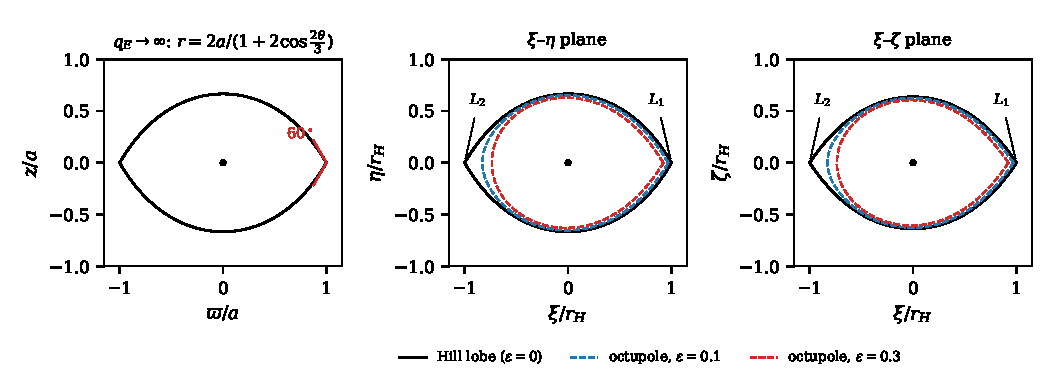
\includegraphics[width=\textwidth]{fig_limits.pdf}
\caption{Exact limiting shapes of the Roche lobe. (a) The dominant-star limit $\qE\to\infty$, equation~(\ref{eq:rlimit}), in a meridional plane; the two hemispheres meet the equator at $60^\circ$. (b,c) The Hill limit $\qE\to0$, equation~(\ref{eq:hillsurf}), in the orbital ($\xi$--$\eta$) and meridional ($\xi$--$\zeta$) planes (solid), together with the lobe of the reduced model $U_0+\epsilon_0 U_1$ of Section~\ref{sec:asym_hill} for $\epsilon_0=r_{\rm H}/a=0.1$ and $0.3$ (dashed). At $\epsilon_0=0.3$ one has $\qE\approx0.09$, well outside the range where the $O(\epsilon_0)$ truncation is controlled; those curves are an illustration of the $L_2$ cap, not a quantitative expansion. The perturbation pins the surface to $L_1$ while lifting it off $L_2$, where the cone becomes a smooth cap of size $\propto\sqrt{\epsilon_0}$.}
\label{fig:limits}
\end{figure*}

\section{Asymptotic expansions}\label{sec:asym}

Both expansions below are regular in the bulk of the lobe and fail in a local region whose geometry supplies the non-analytic term. As $\qE\to\infty$ the outer solution is the rotating-star surface of Section~\ref{sec:limit_inf}, perturbed at $O(\epsilon_\infty^2)$; the singular region is the critical equatorial ring, which produces the logarithm. As $\qE\to0$ the outer solution is the Hill lobe of Section~\ref{sec:limit_hill} plus the octupole; the singular region is the $L_2$ saddle, lifted off the surface, which produces the half-integer power.

\subsection{$\qE\to\infty$: a logarithmic correction}\label{sec:asym_log}

Let $\epsilon_\infty=(3\qE)^{-1/3}$. From equation~(\ref{eq:quintic}), $x_{L_1}=1-\epsilon_\infty+O(\epsilon_\infty^2)$: the inner Lagrange point recedes from the companion by its Hill radius. Substituting into equation~(\ref{eq:psi}) gives the critical potential
\begin{equation}
\Psi_{L_1}=\frac32+\frac92\epsilon_\infty^2+O(\epsilon_\infty^3),
\label{eq:zc}
\end{equation}
which the numerical solution confirms ($[\Psi_{L_1}-3/2]/\epsilon_\infty^2=4.4997$ at $\qE=10^9$). The perturbation of the potential itself, $\qE^{-1}(1/r_2-x)+\tfrac12\qE^{-1}(x^2+y^2)$, is $O(\epsilon_\infty^3)$ except within a distance $O(\epsilon_\infty)$ of the companion, so to $O(\epsilon_\infty^2)$ the lobe is the level set $\Psi_0=\Psi_{L_1}$ of the unperturbed potential, excluding an $O(\epsilon_\infty)$ neighbourhood of the companion where the lobe is cut off by the companion's Hill sphere (volume $O(\epsilon_\infty^3)$, which does not enter the $\epsilon_\infty^2\ln(1/\epsilon_\infty)$ balance). To first order the surface moves inward by $\delta\Psi_{L_1}/|\nabla\Psi_0|$, and
\begin{equation}
\delta V=-\delta\Psi_{L_1}\oint\frac{\dd A}{|\nabla\Psi_0|}.
\label{eq:dV}
\end{equation}
The integral diverges. In the limiting configuration every point of the equator $r=a$, $\theta=\pi/2$ is a critical point of $\Psi_0$: the Hessian of $1/r+\tfrac12r^2\sin^2\theta$ at $(1,0,0)$ is $\operatorname{diag}(3,0,-1)$, with the zero eigenvalue along the equator, so $L_1$ is not an isolated saddle but one point of a critical ring. The same ring makes $\oint\mathrm{d}A/g$ diverge as a single Roche-model star approaches critical rotation; \citet{Paxton2019} fit that divergence along a different path (fixed equatorial radius, varying $\Omega$) as $S\langle g^{-1}\rangle\propto-0.5583\ln(1-\omega^4)$. Their volume at fixed equatorial radius remains finite and is fitted by a polynomial in $\omega$ with no logarithm. The logarithm in $V(c)$ at fixed $\Omega$, which is the binary $\qE\to\infty$ path, is derived below, not fitted. On the limiting surface near the ring, $|\nabla\Psi_0|\simeq2|z|/a$, while the $60^\circ$ cusp gives $\dd A=(2/\sqrt3)\,\dd z\,\dd\varphi$. The integrand behaves as $1/|z|$ and the linearization fails where the displacement $\delta\Psi_{L_1}/|\nabla\Psi_0|\sim\epsilon_\infty^2/|z|$ ceases to be small compared with $|z|$, i.e., for $|z|\lesssim\epsilon_\infty$. Cutting the integral there,
\begin{equation}
\delta V\simeq-\frac92\epsilon_\infty^2\cdot\frac{4\pi}{\sqrt3}\ln\frac1{\epsilon_\infty},
\qquad
\delta\!\left(\frac{\RL}{a}\right)=\frac{\delta V}{4\pi R_0^2},
\end{equation}
and with $\epsilon_\infty^2\ln(1/\epsilon_\infty)=\tfrac13(3\qE)^{-2/3}\ln(3\qE)$,
\begin{equation}
\frac{\RL}{a}=R_0-K\,\frac{\ln\qE}{\qE^{2/3}}-\frac{c_2}{\qE^{2/3}}+O\!\left(\frac{\ln\qE}{\qE}\right),
\label{eq:logexp}
\end{equation}
with
\begin{equation}
K=\frac{3^{-1/6}}{2R_0^2}=0.626\,983\,95 .
\label{eq:K}
\end{equation}
The cutoff determines only $K$. The constant in $c_2$, including the $\ln3$ that comes from writing $\epsilon_\infty^2\ln(1/\epsilon_\infty)$ in terms of $\qE$, is not accessible to it; both coefficients follow from the cylindrical expansion of Appendix~\ref{app:R0}. At a general level $c\ge\tfrac32$ the rotating-star cubic is $(\sin^2\theta/2)\,r^3-cr+1=0$. The substitution $r=(2/\sqrt\kappa)\,s$ with $\kappa=(2c/3)^3$ reduces it to $3s-4s^3=\kappa^{-1/2}\sin\theta$, and the volume element collapses to a regular one-dimensional integral,
\begin{equation}
V(c)=\frac{32\pi}{3\kappa}\int_0^{\pi/2}\frac{\sin\varphi\,\dd\varphi}{\big[3-4\sin^2\!\big(\tfrac13\arcsin(\kappa^{-1/2}\sin\varphi)\big)\big]^3},
\label{eq:Vc}
\end{equation}
and, in cylindrical coordinates with $x=\varpi^2/2$ and $z^2=(c-x)^{-2}-2x$ on the surface, as
\begin{equation}
V(c)=4\pi\int_0^{x_-}\frac{\sqrt{g(x)}}{c-x}\,\dd x,\qquad g(x)=1-2x(c-x)^2,
\label{eq:Vcyl}
\end{equation}
where $x_-(c)$ is the smallest positive root of $g$, the equatorial radius. The cubic $g$ has a double root at $x=\tfrac12$ when $c=\tfrac32$; that double root is the critical ring, and it splits as $\sqrt\delta$ for $c=\tfrac32+\delta$, $\delta=\tfrac92\epsilon_\infty^2$. Appendix~\ref{app:R0} expands equation~(\ref{eq:Vcyl}) about it in closed form:
\begin{equation}
V=V_0+\frac{2\pi}{\sqrt3}\,\delta\ln\delta+\beta\,\delta+o(\delta).
\end{equation}
The logarithmic coefficient reproduces $K$ independently, and
\begin{equation}
\beta=\frac{\pi}{\sqrt3}\Big[10+8\ln(2+\sqrt3)-6\ln6\Big]-\frac{16\pi}{3}=0.993\,058\,876,
\label{eq:beta}
\end{equation}
which Richardson extrapolation of equation~(\ref{eq:Vc}) confirms to 25 digits,
so that
\begin{equation}
\begin{split}
c_2&=-\frac{3^{1/3}}{8R_0^2}\Bigl\{\sqrt3\bigl[10-8\ln2-\tfrac{10}{3}\ln3\\
&\qquad+8\ln(2+\sqrt3)\bigr]-16\Bigr\}=-0.983\,192\,566.
\end{split}
\label{eq:c2}
\end{equation}
With $K$ and $c_2$ fixed, the remainder of the reference solution over $\qE\ge10^3$ is fitted by $\{\qE^{-1}\ln\qE,\qE^{-1},\qE^{-4/3}\ln\qE\}$ to $4\times10^{-4}$, and displacing $c_2$ by $\pm0.04$ degrades this by factors of $3$--$5$.

Two inner regions could have shifted $K$ or produced a further logarithm, and neither does. In the scaled coordinate $Z=z/\epsilon_\infty$ the inner problem on the ring is a regular perturbation whose far-field expansion is a constant plus inverse powers of $Z$; a logarithm in that expansion would generate an $\epsilon_\infty^2\ln^2(1/\epsilon_\infty)$ term or a finite renormalisation of $K$, and $S(\qE)$ of Figure~\ref{fig:asym}a approaches zero with neither. A second inner region surrounds the companion, which sits on the ring: within $O(\epsilon_\infty)$ of it the perturbation $\qE^{-1}(1/r_2-x)$ is comparable to $\delta\Psi_{L_1}$, so the linearisation fails there for a second reason. That region's volume is the companion's Hill sphere, $O(\epsilon_\infty^3)$, and enters $\RL/a$ only at $O(\qE^{-1})$.

Figure~\ref{fig:asym}a tests equation~(\ref{eq:logexp}). Because $c_2$ is known exactly, the combination
\begin{equation}
S(\qE)\equiv\bigl(R_0-\RL/a\bigr)\qE^{2/3}-K\ln\qE-c_2
\end{equation}
must vanish as $\qE^{-1/3}\ln\qE$. The main panel shows that it does; a free fit of the log coefficient is then unnecessary. The inset is the linear combination $(R_0-\RL/a)\qE^{2/3}$ against $\ln\qE$, with slope $K$ and intercept $c_2$. Over $10^4\le\qE\le10^6$ a free fit of the log coefficient still returns $0.641$ against $K=0.627$, and over $10^6$--$10^9$ it returns $0.634$, which is the slow approach of a log series, not a discrepancy in $K$. A basis of integer powers of $\qE^{-1/3}$ without a logarithm fails at the $100\%$ level.

Expanding equation~(\ref{eq:eggleton}) at large $\qE$ gives $0.8167-0.454\,\qE^{-2/3}\ln\qE+\ldots$. Eggleton's $\ln(1+\qE^{1/3})$, introduced to smooth the derivative of Paczy\'nski's piecewise formula, thus has the correct functional form; its coefficient is $28\%$ low and its constant $0.22\%$ high, and the two errors partly cancel over the fitted range. This is the reason a three-coefficient formula from 1983 remains accurate to $1\%$ for all mass ratios.

\subsection{$\qE\to0$: a half-integer power}\label{sec:asym_hill}

In Hill units, with $\epsilon_0\equiv r_{\rm H}/a$, expanding the companion's potential one order beyond the tidal term gives $U=U_0+\epsilon_0 U_1+O(\epsilon_0^2)$, where $U_0$ is equation~(\ref{eq:U0}) and
\begin{equation}
U_1=\tfrac12\left(5\xi^3-3\xi\rho^2\right)
\end{equation}
is the octupole; the centrifugal and quadrupole terms are exact at this order once $\epsilon_0$ is defined through $M_1+M_2$. Write the lobe volume, in units of $r_{\rm H}^3$, as $V/r_{\rm H}^3=V_{\rm H}+\epsilon_0 V_1+\cdots$, with the same dimensionless $V_{\rm H}$ as above.

At $O(\epsilon_0)$ two effects enter. The critical value shifts by $\epsilon_0 U_1(L_1)=\epsilon_0$, and the surface is displaced by $\epsilon_0(U_1-1)/|\nabla U_0|$. Because $U_1$ is odd in $\xi$ while the unperturbed lobe and $|\nabla U_0|$ are even, $\oint U_1\,\dd A/|\nabla U_0|=0$ and only the level shift survives: $V_1=\dd V/\dd c$ at $c=9/2$, the derivative of the enclosed volume with respect to the level. On the critical surface the cubic $3/\rho+\mathcal A\rho^2=c$ gives $\partial\rho/\partial c=\rho^2/[9(\rho-1)]$, whence
\begin{equation}
V_1=-\frac19\oint\frac{\rho^4}{1-\rho}\,\dd\Omega=-1.728\,057\,085\,77,
\label{eq:V1}
\end{equation}
with $\rho(\hat{\bm n})$ from equation~(\ref{eq:hillsurf}); the $1/(1-\rho)$ singularity at the two saddle directions is integrable. Converting with $\epsilon_0=3^{-1/3}t(1+t^3)^{-1/3}$, $t=\qE^{1/3}$,
\begin{equation}
a_1=\frac{3^{-1/3}V_1}{3V_{\rm H}}=-0.264\,750\,47.
\end{equation}

The next term is not $O(\epsilon_0^2)$. At $L_2$ ($\xi=-1$) the octupole {\em lowers} the saddle value by $\epsilon_0$ while the lobe level {\em rises} by $\epsilon_0$, so the perturbed surface no longer passes through $L_2$: the unperturbed cone there becomes a smooth cap. With the Hessian of $U_0$ at $L_2$ equal to $\operatorname{diag}(9,-3,-4)$, the local region is $9s_\xi^2-3s_\eta^2-4s_\zeta^2\ge4\epsilon_0$ in place of the cone $\ge0$, i.e., a hyperboloid of two sheets replacing its asymptotic cone. Linear theory over-removes volume within a distance $\sim\sqrt{\epsilon_0}$ of $L_2$. The linearised displacement is $\epsilon_0(U_1-1)/|\nabla U_0|$: the numerator vanishes at $L_1$ ($U_1=+1$) and equals $-2$ at $L_2$ ($U_1=-1$), so the linearisation is finite at $L_1$ and diverges at $L_2$, and the half-integer power can only come from $L_2$. We define $\Delta V>0$ as the volume restored to the lobe when the linearised surface is replaced by the hyperboloid; Appendix~\ref{app:a32} evaluates
\begin{equation}
\Delta V=\frac{\pi}{3\sqrt3}\int_0^\infty\!\left[w+\frac{2\epsilon_0}{w}-\sqrt{w^2+4\epsilon_0}\right]w\,\dd w=\frac{8\pi}{9\sqrt3}\,\epsilon_0^{3/2},
\label{eq:dV32}
\end{equation}
and
\begin{equation}
a_{3/2}=\frac{3^{-1/2}}{3V_{\rm H}}\cdot\frac{8\pi}{9\sqrt3}=\frac{8\pi}{81V_{\rm H}}=0.205\,681\,47.
\end{equation}
The integrand is the (positive) difference between the linearised and actual transverse radii; the two subtracted pieces are the unperturbed cone, already counted in $V_{\rm H}$, and the $O(\epsilon_0)$ displacement, already counted in $V_1$. At $L_1$ the level set passes through a nondegenerate saddle for every $\epsilon_0$, so the local geometry varies smoothly with $\epsilon_0$ and no half-integer term arises. The same analysis gives the potential difference between the outer and inner Lagrange points of a low-mass secondary, $\Phi_{L_2}-\Phi_{L_1}=\tfrac23\,GM_1/a$ to leading order in $M_1/M_2$ (numerically $0.6667\,GM_1/a$ at $M_2/M_1=10^4$). The expansion is then
\begin{equation}
\frac{\RL}{a}=C\,t\left[1+a_1t+a_{3/2}t^{3/2}+a_2t^2+a_{5/2}t^{5/2}+O(t^3)\right].
\label{eq:hillexp}
\end{equation}
The coefficient $a_{5/2}$ is fitted from the remainder. The coefficient $a_2$ is defined as a Hadamard finite part of an integral over the exact Hill surface; Appendix~\ref{app:a32} shows that the inner matching constant vanishes, so the definition is the $O(\epsilon_0^2)$ volume. Carrying the expansion to $U=U_0+\epsilon_0 U_1+\epsilon_0^2U_2$ with the hexadecapole $U_2=\rho^4P_4(n_\xi)$ and critical level $\tfrac92+\epsilon_0+\tfrac12\epsilon_0^2$, and writing $V/r_{\rm H}^3=V_{\rm H}+V_1\epsilon_0+V_{3/2}\epsilon_0^{3/2}+V_2\epsilon_0^2+\ldots$,
\begin{equation}
a_2=3^{-2/3}\left[\frac{V_2}{3V_{\rm H}}-\frac{V_1^2}{9V_{\rm H}^2}\right],\qquad V_2=V_2^{(U_2)}+V_2^{\rm red}.
\label{eq:a2}
\end{equation}
The hexadecapole enters at first order through a convergent integral over the exact surface,
\begin{equation}
V_2^{(U_2)}=\frac19\oint\frac{\big(\rho^4P_4(n_\xi)-1\big)\rho^4}{1-\rho}\,\dd\Omega=-1.356\,240\,342.
\end{equation}
The octupole enters at second order. Along a ray, with $B=P_3(n_\xi)$, $U_0'=9(\rho_0-1)/\rho_0^2$ and $U_0''=6/\rho_0^3+2\mathcal A$ evaluated on the critical surface, the second-order displacement is $\rho_1=(1-B\rho_0^3)/U_0'$, $\rho_2=-[\tfrac12U_0''\rho_1^2+3B\rho_0^2\rho_1+\tfrac12]/U_0'$, and
\begin{equation}
V_2^{\rm red}=\operatorname{FP}\oint\big(\rho_0^2\rho_2+\rho_0\rho_1^2\big)\,\dd\Omega=-1.260\,674\,456,
\label{eq:V2red}
\end{equation}
where FP denotes the Hadamard finite part with respect to the ray angle $\vartheta$ about the $L_2$ direction. Appendix~\ref{app:a32} shows that the exact ray equation near $L_2$ has a parity under $(\sqrt{\epsilon_0},x)\to(-\sqrt{\epsilon_0},-x)$, with $\rho=1-x$, which fixes the structure of the integrand: multiplied by $\sin\vartheta$ it behaves as $\tfrac23Q^{-3/2}\vartheta^{-2}$ with $Q=3\cos^2\varphi+4\sin^2\varphi$, its $\vartheta^{-1}$ coefficient vanishes identically for every azimuth, and every $O(\epsilon_0^2)$ term of the inner ($L_2$ cap) expansion is a polynomial in the scaled angle whose finite part over $[0,\infty)$ is zero. There is therefore no $\epsilon_0^2\ln\epsilon_0$ term and no inner matching constant, and the finite part in $\vartheta$ is the complete $O(\epsilon_0^2)$ coefficient. The subtraction constant is $\oint\tfrac23Q^{-3/2}\dd\varphi=\tfrac49E(\tfrac14)=0.652\,205\,426$, with $E$ the complete elliptic integral of the second kind with parameter $m=\tfrac14$; a numerical Laurent fit of the integrand returns this value to 15 digits and a $\vartheta^{-1}$ coefficient of $4\times10^{-12}$. We verified the prescription on the pure level shift $U_0\ge\tfrac92+\Delta$, whose $\Delta^2$ coefficient it reproduces to eight digits against the exact volume function of the Hill potential. Altogether
\begin{equation}
a_2=-0.348\,082,
\end{equation}
from the finite-part quadrature, independent of the matching radius to $10^{-9}$. Fixing $a_1$ and $a_{3/2}$ and fitting $a_2$ over $10^{-9}\le\qE\le10^{-4}$ recovers $-0.346$ with a $\{t^2,t^{5/2},t^3\}$ basis and $-0.348$ with one more half-integer term: an independent determination at $10^{-3}$, not six figures. The six figures remain the quadrature. An independent check is the reduced-model volume $U_0+\epsilon_0 U_1$. Subtracting the known $V_{\rm H}$, $V_1$ and $a_{3/2}$ terms and dividing by $\epsilon_0^2$ leaves a remainder that approaches $V_2^{\rm red}$ as $\sqrt{\epsilon_0}\to0$. The volumes at quadrature orders $n=90$ and $n=200$ agree to $10^{-14}$ for $\epsilon_0\ge10^{-5}$ and are included with the source. Richardson extrapolation of that remainder in powers of $\sqrt{\epsilon_0}$ over $10^{-3}\ge\epsilon_0\ge10^{-5}$ returns $-1.2605$ with a spread of $5\times10^{-4}$ among polynomial degrees; cancellation grows below $\epsilon_0\approx2\times10^{-6}$. The reduced model therefore confirms four digits of the finite-part value, which is the more precise evaluation. That spread propagates as $\delta a_2\simeq0.11\,\delta V_2^{\rm red}\approx5\times10^{-5}$, consistent with the finite-part quadrature at that level; the six figures of $a_2$ come from that quadrature, stable to $10^{-9}$ against the matching radius. With $a_1$, $a_{3/2}$ and $a_2$ fixed, the reference solution over $10^{-9}\le\qE\le10^{-4}$ leaves a remainder fitted by $\{t^{5/2},t^3,t^{7/2}\}$ to $4\times10^{-7}$, with $a_{5/2}\simeq0.417$. Through $t^{5/2}$, equation~(\ref{eq:hillexp}) is good to $5\times10^{-5}$ relative at $\qE=10^{-4}$ and $5\times10^{-7}$ at $10^{-6}$. The two-term log expansion, equation~(\ref{eq:logexp}), is good to $2\times10^{-4}$ at $\qE=10^{4}$ and $7\times10^{-6}$ at $10^{6}$.

Two tests of $a_{3/2}$ were made. In the reduced model $U_0+\epsilon_0 U_1$, $[V-V_{\rm H}-\epsilon_0 V_1]/\epsilon_0^{3/2}$ evaluates to $1.5146$, $1.5757$, $1.6000$, $1.6083$ at $\epsilon_0=10^{-2},10^{-3},10^{-4},10^{-5}$, converging on $8\pi/(9\sqrt3)=1.6123$ with the $\sqrt{\epsilon_0}$ drift expected from the next term. In the full Roche problem (Figure~\ref{fig:asym}b), 19 reference values over $10^{-9}\le\qE\le10^{-4}$ fitted with integer powers only give residuals of $2\%$ of the signal and a spurious $a_1=-0.254$; a free fit including $t^{3/2}$ and $t^{5/2}$ returns $a_1=-0.2647$ and $a_{3/2}=0.202$.

\begin{figure*}
\centering
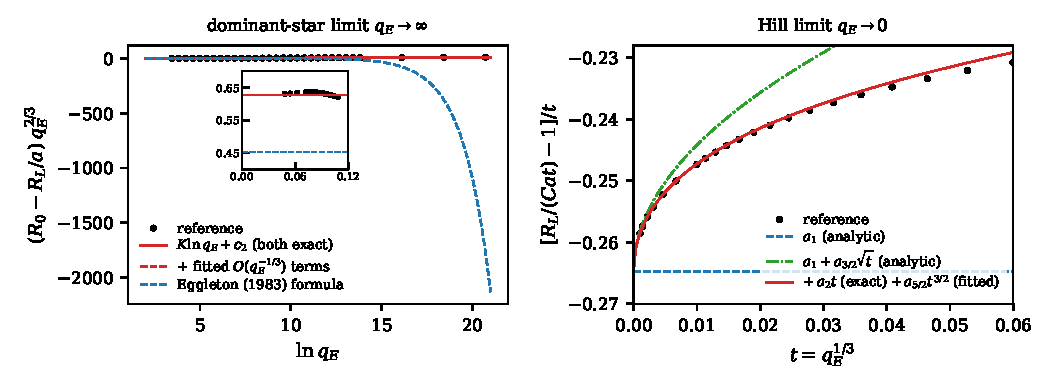
\includegraphics[width=\textwidth]{fig_asymptotics.pdf}
\caption{Asymptotic structure of the reference solution. (a)~Dominant-star limit: $S(\qE)=(R_0-\RL/a)\qE^{2/3}-K\ln\qE-c_2$ against $\qE^{-1/3}\ln\qE$, which vanishes as required. Inset: $(R_0-\RL/a)\qE^{2/3}$ against $\ln\qE$ is linear with the exact slope $K$ and intercept $c_2$ of equation~(\ref{eq:logexp}); the dashed curve adds the two fitted $O(\qE^{-1/3})$ terms. (b)~Hill limit: $[\RL/(Cat)-1]/t$ against $t=\qE^{1/3}$ approaches the analytic $a_1$ with the $\sqrt t$ dependence produced by the $L_2$ cap; the solid curve adds the quadrature $a_2$ and the fitted $a_{5/2}$ of equation~(\ref{eq:hillexp}).}
\label{fig:asym}
\end{figure*}

Both ends of the mass-ratio range are therefore non-analytic in $\qE^{1/3}$, for different geometric reasons: a ring of critical points at one end, a single critical point being lifted off the surface at the other. No rational-plus-logarithm formula of the Eggleton family can reproduce either beyond leading order, which is of no practical consequence at the $10^{-4}$ level but explains, from a second direction, why refits with free exponents go wrong: they attempt to mimic non-analytic behavior with the wrong non-analyticity.

\section{Reference solution}\label{sec:num}

\subsection{Method}

The inner lobe of $M_1$ is star-shaped from $M_1$: for every $\qE$ we have tested, $\Psi>\Psi_{L_1}$ at interior samples out to the first root, $\partial_R\Psi$ never increases along that segment, and the first root always lies in $(0,x_{L_1}]$. Further crossings of $\Psi=\Psi_{L_1}$ exist on rays that continue toward $M_2$; they belong to the companion's lobe and lie beyond the first root. For each direction $(\theta,\varphi)$ the lobe radius is therefore that first root, obtained by a coarse scan followed by 70 bisection steps in 80-bit extended precision; $x_{L_1}$ is polished by Newton iteration to the same precision. The volume $V=\tfrac13\oint R^3\dd\Omega$ is evaluated over one octant by composite Gauss--Legendre quadrature. Panel half-width about the $L_1$ direction is $d=\min(4\epsilon_\infty,0.9\pi/2)$, with $\epsilon_\infty$ itself capped at $0.4$, so that the conical point of the surface at $L_1$ lies at a panel corner; for $\qE\lesssim5$ the $0.9\pi/2$ cap is active and the $4\epsilon_\infty$ refinement without the cap is used only for $\qE\gtrsim10$. The integrand is $R^3\sin\theta$ with $R$ Lipschitz, and near $L_1$ one has $R\simeq x_{L_1}-c\vartheta$, so the kink is in the derivative of a function whose value is almost constant; product Gauss--Legendre clusters nodes at the panel edges, which is where the kink sits. At large $\qE$ the offending panel is itself small (solid angle $O(\epsilon_\infty^2)$). The surface integral of $|\geff|$ in equation~(\ref{eq:vz}) is evaluated on the same nodes using $\dd A=R^2\sin\theta\,\dd\theta\,\dd\varphi\,|\nabla\Psi|/(-\partial_R\Psi)$, and the volume is recovered independently from it.

\subsection{Accuracy}

Table~\ref{tab:converge} in Appendix~\ref{app:tables} gives the convergence ladder. A double-precision ladder at $n=20$, $40$ and $80$ gives observed order $p\simeq5.9$ at $\qE=1$: high algebraic order, not spectral, already at $10^{-13}$ by $n=100$ ($|\Delta R|_{100\to200}=3\times10^{-13}$). Between $n=200$ and $n=400$ the volume-equivalent radius changes by at most $5\times10^{-15}$, and the direct volume agrees with the value recovered from equation~(\ref{eq:vz}), an entirely different functional of the same surface, to $\le10^{-14}$ at every mass ratio tested. The reference table (Table~\ref{tab:ref}) was computed with $n=300$, a few hours on a single core. The estimated absolute numerical error in $\RL/a$, conservatively assessed as the larger of the $n=200\to400$ change and the von~Zeipel residual at $n=400$, is below $10^{-13}$ at every mass ratio in Table~\ref{tab:converge}, which is 13 significant figures near $\qE\sim1$ and at least 10 significant figures at $\qE=10^{-6}$, where $\RL/a\sim5\times10^{-3}$. Neither diagnostic is a rigorous bound on the discretization error; both are the standard estimates, and they agree. At $\qE=10^{4}$ and $10^{6}$ the $200\to400$ change exceeds the $100\to200$ change, which is a round-off floor rather than discretisation convergence: the error estimate there is a round-off estimate, not a truncation estimate. The two exact limits, equations~(\ref{eq:R0}) and (\ref{eq:C}), and the exact log coefficient of Section~\ref{sec:asym_log} provide checks that are independent of the code.

Comparison with published values: at $\qE=1$ our $\RL/a=0.379\,863\,240\,9274$ agrees with the $0.379\,863$ of \citet{Mochnacki1984} to all six of his digits; the ten equatorial radii $R(90^\circ,\varphi)$ tabulated by \citet{LeahyLeahy2015} for $\qE=1$ are reproduced to $\le5\times10^{-8}$, their stated root tolerance; and all eight finite entries of Table~1 of \citet{Eggleton1983}, including $r_L(\infty)=0.8149$, agree with our values to his four printed digits. Mochnacki's $x_{L_1}=0.71751$ at $M_2/M_1=0.10$ satisfies equation~(\ref{eq:seidov}) to $1$ part in $10^5$.

\subsection{Reference table and lobe geometry}\label{sec:table}

Table~\ref{tab:ref} lists $\RL/a$, $\RL/r_{\rm H}$ and $x_{L_1}/a$ at half-decade intervals, with $r_{\rm H}/a=[\qE/(3(1+\qE))]^{1/3}$; the full table at 73 mass ratios, and the logarithmic derivative $D=\partial\ln(\RL/a)/\partial\ln\qE$ at 49 mass ratios (\texttt{derivative\_reference.txt}), are provided in machine-readable form. The exact symmetry $x_{L_1}(\qE)+x_{L_1}(1/\qE)=1$ holds to the last printed digit. Figure~\ref{fig:sections} shows cross-sections of the lobe in the orbital and meridional planes, with both exact limits overlaid.

\begin{figure*}
\centering
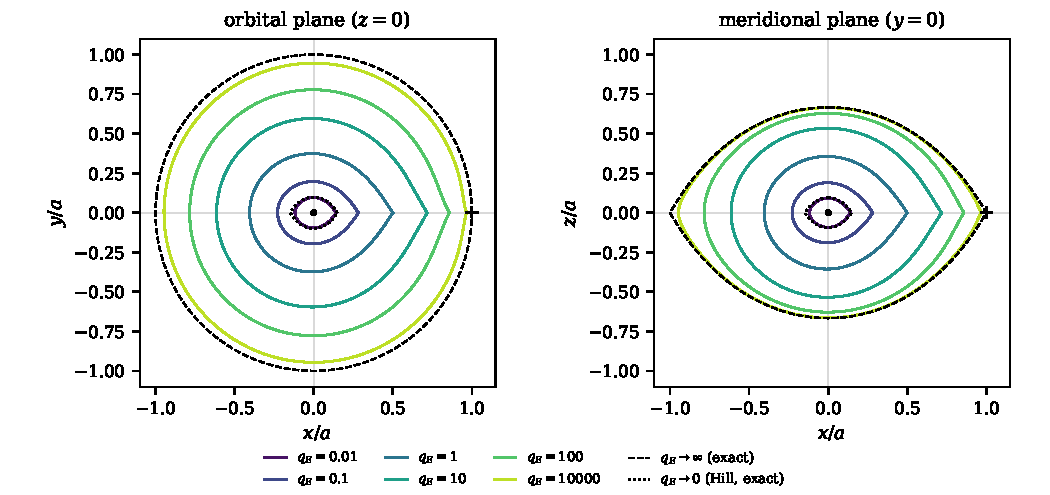
\includegraphics[width=\textwidth]{fig_sections.pdf}
\caption{Cross-sections of the Roche lobe of $M_1$ (at the origin; $M_2$ at the cross) in the orbital plane (left) and the meridional plane containing the binary axis (right), for $\qE=M_1/M_2$ from $10^{-2}$ to $10^4$. The dashed curve is the exact $\qE\to\infty$ surface of equation~(\ref{eq:rlimit}), a unit circle in the orbital plane; the dotted curve is the exact Hill surface of equation~(\ref{eq:hillsurf}), scaled to the Hill radius at $\qE=10^{-2}$. Lengths in units of the separation.}
\label{fig:sections}
\end{figure*}

\section{Approximation formulae}\label{sec:fits}

\subsection{Existing formulae over twelve decades}

Table~\ref{tab:fits} and Figure~\ref{fig:fits} compare three published formulae with the reference solution over $10^{-6}\le\qE\le10^6$. The Eggleton formula has a maximum error of $0.83\%$ and an rms error of $0.42\%$, consistent with his claim of better than $1\%$, and it retains this accuracy without limit at both ends because its exponents are the correct $2/3$ and $1/3$.

\begin{figure*}
\centering
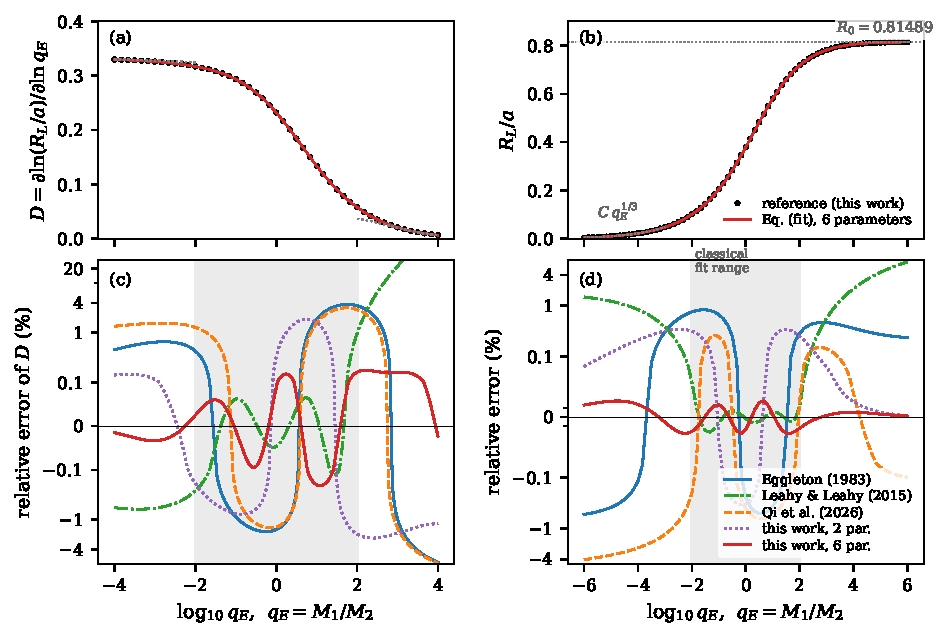
\includegraphics[width=\textwidth]{fig_fits_deriv.pdf}
\caption{(a,c)~Logarithmic derivative $D=\partial\ln(\RL/a)/\partial\ln\qE$. (b,d)~Volume-equivalent radius $\RL/a$. Top: reference solution (points) and equation~(\ref{eq:fit}) with (\ref{eq:h6}) (curve). Dotted lines in (a) are the asymptotic forms of Sections~\ref{sec:asym_log} and~\ref{sec:asym_hill}, drawn only at the ends; in (b) they are the exact limits $R_0$ and $C\qE^{1/3}$. Bottom: relative errors of the published formulae and of the two new ones (note the symmetric-log scale in (c) and (d)). The shaded band marks $0.01\le\qE\le100$.}
\label{fig:fits}
\end{figure*}

\citet{LeahyLeahy2015} generalized equation~(\ref{eq:eggleton}) to $a_1q^{a_4}/[a_2q^{a_5}+\ln(1+a_3q^{a_4+1/3})]$ with their $q=M_2/M_1=1/\qE$ and fitted it over $0.01\le q\le100$ ($10^{-2}\le\qE\le10^{2}$). The published coefficients are $a_1=0.64334$, $a_2=0.86907$, $a_3=1.2809$, $a_4=-0.74303$ and $a_5=+0.73103$. With that $a_5$ the formula is wrong by orders of magnitude except at $q=1$, where $q^{a_5}=1$ independently of the sign, and the stated large-$q$ limit is recovered only if $a_5<0$; with $a_5=-0.73103$ it reproduces our reference values to $0.038\%$ over the calibrated range, so the published sign is a typographical error. They do not print a table of $R_{\rm eq}(q)$. Against their own stated rms of $2.2\times10^{-5}$ (absolute, in units of $a$, on $\sim150$ numerical points), the published sign fails by orders of magnitude, while the flipped sign recovers that accuracy (rms $2.7\times10^{-5}$ against our table over the same interval). At $q=1$ the flipped formula returns $0.379856$, against Mochnacki's $0.379863$. We find no published erratum. Outside that range, however, the free exponents $a_4=-0.743$ and $a_5=-0.731$ imply $\RL\propto\qE^{+0.012}$ as $\qE\to\infty$, so the formula diverges instead of approaching $R_0$; the error is $2.2\%$ at $\qE=10^4$ and $7.3\%$ at $10^6$, and $1.5\%$ at $\qE=10^{-6}$. The $+22\%$ derivative error at $\qE=10^3$ in Table~\ref{tab:deriv} lies outside their calibration and is a consequence of that divergence, not of the mid-range fit.

\citet{Qi2026} refitted equation~(\ref{eq:eggleton}) as
\begin{equation}
\frac{\RL}{a}=\frac{0.49\,\qE^{0.665}}{0.602\,\qE^{0.665}+\ln\!\left(1+\qE^{0.329}\right)},
\label{eq:qi}
\end{equation}
four coefficients (they write the same expression in $q=M_2/M_1=1/\qE$). Over $0.01\le\qE\le100$ this gives a maximum error of $0.65\%$. At small $\qE$ the formula scales as $\qE^{0.336}$ rather than $\qE^{1/3}$, so it underestimates $\RL$ without limit as a fraction of the truth: $\RL/(a\qE^{1/3})\propto\qE^{0.002667}\to0$. With the signed relative-error convention $\RL^{\rm fit}/\RL^{\rm ref}-1$ used throughout, the error tends to $-1$ and is therefore bounded; the inverse ratio $\RL^{\rm ref}/\RL^{\rm fit}$ diverges. Over the sampled interval the signed error is $-1.3\%$ at $\qE=10^{-3}$, $-2.4\%$ at $10^{-4}$ and $-4.1\%$ at $10^{-6}$. These are the mass ratios of a Jupiter-, Neptune- and sub-Earth-mass planet around a solar-mass star, a regime in which the Roche-lobe radius is used routinely (planetary tidal disruption and mass loss, and extreme-mass-ratio compact binaries), and one in which the original Eggleton formula is more accurate than either refit.

\subsection{Formulae with exact asymptotics}

Both failures have the same cause: the exponents of an Eggleton-type formula are not free parameters but are fixed by the exact scalings, and the coefficients multiplying the leading terms are fixed by $R_0$, $K$ and $C$. Writing $t=\qE^{1/3}$, the form
\begin{equation}
\frac{\RL}{a}=\frac{R_0\,A\,t^2}{A\,t^2+R_0\ln(1+E\,t)+h(t)},
\label{eq:fit}
\end{equation}
with
\begin{equation}
A=\frac{R_0^2}{3K}=\tfrac23\,3^{1/6}R_0^4=0.353\,033\,3,\qquad E=\frac AC=0.715\,647\,4,
\end{equation}
reproduces $R_0$, the exact log coefficient $K$, and $C$ for any $h(t)$ that is $O(t^2)$ as $t\to0$ and tends to a constant as $t\to\infty$. With $h\equiv0$ this is Eggleton's form with the asymptotically correct coefficients $(0.353,0.433,0.716)$ in place of $(0.49,0.6,1)$; it is exact at both ends but $4.5\%$ low at $\qE=1$, which shows that Eggleton's coefficients are a compromise that trades the limits for the middle. The freedom in $h$ restores the middle without disturbing the ends. Minimizing the maximum relative error over the 73 reference values gives, with two free coefficients,
\begin{equation}
h(t)=\frac{H\,t^2}{1+J\,t^2},\qquad H=-0.038\,141,\quad J=0.154\,401,
\label{eq:h2}
\end{equation}
with maximum error $0.345\%$, and with six,
\begin{equation}
h(t)=\frac{H\,t^2}{1+Jt^2}+\frac{H_2\,t^3}{(1+J_2t^2)^{3/2}}+\frac{H_3\,t^4}{(1+J_3t^2)^{2}},
\label{eq:h6}
\end{equation}
\begin{equation}
\begin{aligned}
H&=-0.007\,259, & J&=0.061\,923,\\
H_2&=-0.130\,971, & J_2&=0.707\,426,\\
H_3&=\phantom{-}0.134\,476, & J_3&=1.114\,754,
\end{aligned}
\end{equation}
with maximum error $0.018\%$ and rms error $0.011\%$ over $10^{-6}\le\qE\le10^6$ (Figure~\ref{fig:fits}). The coefficients are a least-squares start followed by six Nelder--Mead rounds on the maximum relative error over the 73 reference values, not a Remez exchange and not a global search. The residual has five near-equal peaks at $0.0178\%$ ($\qE\approx1.5\times10^{-5}$, $4.6\times10^{-3}$, $0.68$, $4.6$ and $46$) and a weaker sixth at $0.014\%$ ($\qE\approx0.10$). We therefore report $0.018\%$ as the maximum error of this fit, an upper bound on the achievable minimax for this functional form. Re-evaluating on a $10^4$-point cubic spline of that table, log-spaced over the same twelve decades, returns a continuum maximum of $0.018\%$. The two-coefficient continuum maximum is $0.345\%$ at $\qE=29$. Rounding the coefficients to four significant figures does not change these numbers. The denominator of equation~(\ref{eq:fit}) with (\ref{eq:h6}) is positive and strictly increasing on a $2\times10^4$-point log grid $10^{-18}\le\qE\le10^{12}$, with no pole. Each $|h|$ term is bounded ($|H|/J=0.117$, $|H_2|/J_2^{3/2}=0.220$, $|H_3|/J_3^2=0.108$); their sum $0.446$ is less than $R_0$, and $At^2+R_0\ln(1+Et)$ dominates at both ends. That is a numerical check plus a bound, not a formal proof of monotonicity. As $t\to0$ the denominator behaves as $R_0 E t$. Appendix~\ref{app:code} collects a short implementation.

The form does not enforce the sub-leading coefficients we derived. Expanding equation~(\ref{eq:fit}) at small $t$ gives $a_1^{\rm fit}=E/2-(A+H)/(R_0 E)$, which with the six-coefficient $H$ is $-0.235$ rather than the exact $-0.2648$; the omitted $t^{3/2}$ term is absorbed inside the calibrated range. At large $t$ the intercept is set by $h(\infty)$: the fit does not enforce the exact subleading coefficient, and its implied value $c_2^{\rm fit}=3K[\ln E+h(\infty)/R_0]=-1.16$ differs from the asymptotic $-0.983$ by $18\%$, a difference absorbed by the fitted $O(\qE^{-1})$ terms inside the calibrated range. One could fix $H$ so that $a_1$ is exact and add a term $\propto t^{7/2}/(1+Jt^2)^{7/4}$ that reproduces $a_{3/2}$, making $h(t)$ exact through second order at both ends. We do not: those constraints spend the remaining freedom on the extreme ends, already correct to leading order, at the expense of $10^{-4}\lesssim\qE\lesssim10^4$, where the formula is used. The practical gain at the $10^{-4}$ level is negligible. We regard the present fit, exact at leading order at both ends and accurate to $0.018\%$ where binaries live, as the more useful end point.

Beyond the fitted range the six-coefficient formula follows the asymptotic series of equations~(\ref{eq:logexp}) and (\ref{eq:hillexp}) to five or six digits at $\qE=10^{\pm9}$, where the Eggleton formula is off by $0.2\%$ and $0.7\%$ and the two refits by much more. Equation~(\ref{eq:fit}) with (\ref{eq:h6}) is therefore the most accurate globally valid closed-form formula among those compared here, both inside and outside the classical range, and is the only one with correct limiting behavior. \citet{LeahyLeahy2015} also published a cubic spline in $\log q$ on 28 nodes over $0.01\le q\le100$, with rms $1.4\times10^{-7}$ in $R_{\rm eq}$, the same volume-equivalent radius, quoted as an absolute residual in units of the separation (relative $\sim4\times10^{-7}$ near $q=1$); that interpolation is substantially more accurate within its calibrated interval, but it is neither global nor asymptotically constrained. The two-coefficient version offers Eggleton-level simplicity with exact limits and $2.4$ times smaller error.

\subsection{Derivatives and mass-transfer stability}\label{sec:deriv}

Whether Roche-lobe overflow is dynamically stable is decided by comparing the donor's adiabatic response $\zeta_{\rm ad}=\partial\ln R_\ast/\partial\ln M_{\rm d}$ with the lobe's logarithmic response $\zeta_L=\partial\ln\RL/\partial\ln M_{\rm d}$ \citep{HjellmingWebbink1987,Soberman1997}. Codes that adopt a fitting formula therefore need its derivative, not only its value.

For conservative transfer with donor $M_1$ (so $\qE=M_{\rm d}/M_{\rm a}$), $a\propto(M_1M_2)^{-2}$ at fixed total mass and angular momentum and $\partial\ln\qE/\partial\ln M_1=1+\qE$, so
\begin{equation}
\zeta_L=(1+\qE)\,D+2(\qE-1),\qquad D\equiv\frac{\partial\ln(\RL/a)}{\partial\ln\qE}.
\label{eq:zetaL}
\end{equation}
We compute $D$ from the reference solution by central differences in $\ln\qE$ with step $\delta=5\times10^{-3}$; repeating at $\delta/2$ for $\qE=0.1$, $1$ and $10$ changes $D$ by at most $3\times10^{-8}$. Eggleton's error in $D$ reaches $7.4\%$ over $10^{-4}\le\qE\le10^4$ and $3.7\%$ over $0.01\le\qE\le100$, several times his error in the value, and it oscillates in sign (Figure~\ref{fig:fits}, Table~\ref{tab:deriv}). The six-parameter formula holds the derivative error to $0.20\%$ or smaller.

The analysis is for fully conservative transfer. For non-conservative transfer $\zeta_L$ acquires terms from the mass-loss fraction and the specific angular momentum of the ejected material \citep{Soberman1997}, but $D$ still enters through the lobe term, and that term still dominates for low-mass convective donors. The ranking therefore survives. The modern determination of $\qE^{\rm crit}$ for convective donors is set by $\zeta_{\rm ad}$, not by the fitting formula: adiabatic sequences give a spread of tens of percent \citep{Ge2010,Ge2015,Ge2020,Pavlovskii2015,WoodsIvanova2011,Temmink2023}. A $0.5\%$ shift from Eggleton versus the present formula lies far below that. Population-synthesis codes evaluate the lobe through Eggleton \citep{Hurley2002}; the common-envelope energy formula is that of \citet{Webbink1984}. Paczy\'nski's coefficient, not Eggleton, is the one that entered the cataclysmic-variable angular-momentum-loss work of \citet{Rappaport1983}.

The critical mass ratio $\qE^{\rm crit}$ at which $\zeta_L=\zeta_{\rm ad}$ shifts by at most $0.52\%$ if Eggleton's formula is used, at the fully convective value $\zeta_{\rm ad}=-1/3$; at the radiative-envelope value $\zeta_{\rm ad}=6.85$ of \citet{HjellmingWebbink1987} the shift is $0.01\%$ (Table~\ref{tab:qcrit}). Equation~(\ref{eq:fit}) with (\ref{eq:h6}) moves $\qE^{\rm crit}$ by less than $0.03\%$ for every $\zeta_{\rm ad}$ we compute. Once $\qE\gtrsim1$ the orbital term $2(\qE-1)$ dominates $\zeta_L$, so a few-percent error in $D$ does not move the radiative stability boundary by a comparable fraction.

\begin{deluxetable*}{lcccccc}
\centerwidetable
\tablewidth{\textwidth}
\tablecaption{Accuracy of approximation formulae against the reference solution.\label{tab:fits}}
\tablehead{\colhead{Formula} & \colhead{Free coeff.} & \colhead{max $|\delta|$\tablenotemark{b}} & \colhead{max $|\delta|$\tablenotemark{c}} & \colhead{rms $|\delta|$\tablenotemark{c}} & \colhead{$\lim_{\qE\to\infty}$} & \colhead{$\lim_{\qE\to0}\RL/(a\qE^{1/3})$}}
\startdata
\citet{Eggleton1983}      & 3 & $0.83\%$  & $0.83\%$ & $0.42\%$  & $0.8167$ & $0.490$ \\
\citet{LeahyLeahy2015}\tablenotemark{a} & 5 & $0.038\%$ & $7.3\%$  & $2.2\%$   & diverges & $0.502$ \\
\citet{Qi2026}            & 4 & $0.65\%$  & $4.1\%$  & $1.5\%$   & $0.8140$ & $0$ \\
This work, eq.~(\ref{eq:fit}) with (\ref{eq:h2}) & 2 & $0.345\%$  & $0.345\%$ & $0.20\%$  & $R_0$ (exact) & $C$ (exact) \\
This work, eq.~(\ref{eq:fit}) with (\ref{eq:h6}) & 6 & $0.018\%$ & $0.018\%$ & $0.011\%$ & $R_0$ (exact) & $C$ (exact) \\
\hline
Exact                     &   &           &          &           & $0.81489$ & $0.49331$ \\
\enddata
\tablecomments{$^{a}$With $a_5=-0.73103$; see text.\hfill $^{b}$Over $0.01\le\qE\le100$.\hfill $^{c}$Over $10^{-6}\le\qE\le10^{6}$.}
\end{deluxetable*}

\section{Discussion}\label{sec:disc}

The expansion of $\RL(\qE)$ is not a power series in $\qE^{1/3}$ at either end: a logarithm as $\qE\to\infty$ (the equator of the limiting surface is a {\em ring} of critical points) and a half-integer power as $\qE\to0$ (a single critical point, $L_2$, is lifted off the surface). Eggleton's $\ln(1+\qE^{1/3})$, introduced in 1983 only to smooth a derivative, has the correct logarithmic structure with a coefficient $28\%$ low ($0.454$ versus the exact $K=0.627$) and a limit $0.2\%$ high; the two errors partly cancel. This is why three coefficients hold to $1\%$ for all mass ratios and extrapolate safely, and why fits that free the exponents cannot: they replace the true non-analyticity with the wrong one. For any Roche-type fit we therefore fix the exponents at $2/3$ and $1/3$, keep the logarithm, and fit only a correction that vanishes at both ends. \citet{Dermine2009} is the existing example: they generalise equation~(\ref{eq:eggleton}) to radiation pressure by keeping those exponents and fitting only $A(f)$, $B(f)$ and $C(f)$. The same construction applies to eccentric and asynchronous lobes \citep{Sepinsky2007} and to Yukawa and power-law gravity \citep{Velasquez2026}.

Formulae accurate to $0.3\%$ in $\RL/a$ are accurate to only a few percent in $D=\partial\ln(\RL/a)/\partial\ln\qE$, and it is $D$ that sets mass-transfer stability. Eggleton's $D$ has a maximum error of $3.7\%$ over $0.01\le\qE\le100$ ($7.4\%$ over eight decades), changes sign across the classical range, and is several times his error in the value ($-1.60\%$ versus $-0.25\%$ at $\qE=1$). For conservative transfer $\zeta_L=(1+\qE)D+2(\qE-1)$, and once $\qE\gtrsim1$ the orbital term dominates, so the radiative-donor boundary ($\zeta_{\rm ad}=6.85$) moves by only $0.01\%$ while the fully convective boundary ($\zeta_{\rm ad}=-1/3$, $\qE^{\rm crit}=0.63$) moves by $0.5\%$. The derivative error therefore matters most where the lobe term dominates: low-mass, convective donors (CVs, LMXBs, and planet or brown-dwarf donors). The six-coefficient formula reduces the derivative error to $0.2\%$ and the $\qE^{\rm crit}$ shifts to $\le0.02\%$. That $0.5\%$ convective-boundary shift is far smaller than the uncertainty in $\zeta_{\rm ad}$.

The planetary and extreme-mass-ratio regime has been served by the wrong numbers. The Paczy\'nski coefficient $0.462\,24$, still widely used for planets, is exactly $\tfrac23 r_{\rm H}$, the $\eta$-axis (side) radius of the Hill lobe, and is $6.3\%$ below the exact asymptote $C=0.493\,31$; a planet of Jupiter's mean density fills its lobe at $P=8.27$~h, not $9.12$~h, and the critical density for tidal disruption at fixed separation shifts by $22\%$ ($(C/0.46224)^3=1.215$). Both modern refits are {\em worse} than Eggleton for $\qE\lesssim10^{-3}$: \citet{Qi2026} underestimate the lobe by $1.3\%$ for a Jupiter and $2.7\%$ for a Neptune around a Sun, and by $3.1\%$ for a $0.2\,M_\odot$ white dwarf around a $10^4\,M_\odot$ intermediate-mass black hole, a $4.7\%$ error in the gravitational-wave frequency at overflow onset. That $4.7\%$ is a comparison between Newtonian Roche-lobe prescriptions. At overflow the Newtonian separation is tens of gravitational radii for these masses ($z=2(M_1+M_2)/a\approx0.03$ for a $0.02\,R_\odot$, $0.2\,M_\odot$ white dwarf around $10^4\,M_\odot$). \citet{Ratkovic2005}, an unrefereed preprint, treat the second post-Newtonian Roche problem with a three-body Lagrangian valid near the less massive star. They write the volume-equivalent radius as Eggleton's $Q(q)$ times a correction factor $C(q,z)=1+z(1.951\,q^{1/5}-1.812)$. Their figures at $z=0.2$ and $0.4$ show $20$--$30\%$ corrections at low mass ratio; at the overflow $z$ of the IMBH--WD example that fit gives a $4\%$ correction, comparable to the difference between the Newtonian formulae. The construction does not apply near the more massive body. The exact Hill-lobe surface gives the lobe extent in every direction, with a caveat at planetary mass ratios: at $\qE\sim10^{-3}$ the $O(t)$ correction to $\RL/a$ is $2.6\%$, so directional radii taken from the $\epsilon_0=0$ surface are uncertain at the percent level. For WASP-12b we therefore use the full Roche solution at the observed mass ratio. Adopting $M_p=1.47\,M_{\rm J}$, $M_\ast=1.434\,M_\odot$, $a=0.02340$~AU and $R_p=1.90\,R_{\rm J}$ \citep{Collins2017}, one has $\qE=9.79\times10^{-4}$ and $\RL=2.35\,R_{\rm J}$. The optical transit radius is wavelength- and model-dependent: \citet{Hebb2009} had $1.79\,R_{\rm J}$, the value used by \citet{Lai2010}, and \citet{Vissapragada2026} adopt $2.0\,R_{\rm J}$. With $R_p=1.90\,R_{\rm J}$ the planet fills $81\%$ of the volume-equivalent radius and $90\%$ of the polar extent ($2.12\,R_{\rm J}$). Published fill factors for this system are not the same quantity. \citet{Lai2010} take $R_L=a(q/3)^{1/3}=1.85\,R_p$ (the Hill sphere; fill $54\%$) and $y_L=(2/3)x_L=1.23\,R_p$ (Paczy\'nski's $\eta$-axis); \citet{Vissapragada2026} quote $R_p/R_{\rm Roche}=(R_p/a)(M_p/3M_\ast)^{-1/3}=0.55$, the same Hill-sphere ratio. The Hill-sphere fill $55\%$ and the volume-equivalent fill $81\%$ differ by $\kappa^{-1}\simeq1.41$, which is the point of Section~\ref{sec:limit_hill}. We quote the polar extent because it is the smallest of the lobe's axial extents and the one a transit radius, which measures the sky-projected cross-section, is most directly compared with; it is a conservative geometric comparison, not the overflow direction. Overflow itself proceeds through $L_1$ along the star--planet axis, where the lobe extends farthest. Those fill factors compare a measured transit radius with the Roche geometry. Roche-lobe contact in the binary-star sense is $\RL$ reaching the stellar radius; a fluid body can shed mass through $L_1$ from a smaller volume fill factor if it is distorted, or remain bound at a larger fill factor if it is centrally condensed. The exact treatment changes the number that should be compared with a transit radius; it does not change the conclusion that the planet is close to, and not clearly overflowing, the lobe.

The expansions themselves are a Newtonian point-mass construction, pushed here over $10^{-6}\le\qE\le10^6$. The small-$\qE$ end is the regime of planets and of white-dwarf companions to intermediate-mass black holes, where the Roche formalism is used and the Hill surface is the right leading-order geometry. The large-$\qE$ end is the Roche-model rotating star: the lobe of $M_1$ fills $0.815a$, which is the critical surface already used in stellar-structure codes \citep{Paxton2019,Maeder2009}. The point-mass idealisation for $M_1$ is that model's premise, not a new one, and the binary logarithm computed here is the first correction from a light companion. At $\qE=10^{6}$ that companion is a planet or brown dwarf.

This is the regime in which Roche-lobe formulae are now used most and tested least: planet engulfment, evaporating hot Jupiters, and white-dwarf companions to intermediate-mass black holes in the {\em LISA} band.

\section{Summary}\label{sec:summary}

\begin{enumerate}
\item The $L_1$ quintic has Galois group $S_5$ for generic rational mass ratio, so $x_{L_1}$ has no expression in radicals; infinitely many rational mass ratios, given by Seidov's inversion, have rational $L_1$.
\item In the dominant-star limit the lobe is the critical rotating-star surface $r=2a/(1+2\cos\tfrac{2\theta}{3})$, and its volume-equivalent radius is the closed form of \citet{Kopal1959}, $R_0=[3\sqrt3-4+3\ln(6-3\sqrt3)]^{1/3}a=0.814\,885\,68\,a$.
\item The leading correction to $R_0$ is $-K\qE^{-2/3}\ln\qE$ with $K=3^{-1/6}/(2R_0^2)$ exactly, and the next coefficient $c_2=-0.98319$ is given in closed form by equation~(\ref{eq:c2}); the logarithm arises because the equator of the limiting surface is a ring of critical points. The Eggleton formula has this structure with a $28\%$ smaller coefficient, which explains its robustness.
\item In the Hill limit the lobe surface is $\rho=(2/m)\sin(\tfrac13\arcsin m)$ exactly, $\RL\to0.711\,470\,70\,r_{\rm H}=0.493\,306\,23\,a\,\qE^{1/3}$, and the expansion contains a $t^{3/2}$ term with coefficient $8\pi/(81V_{\rm H})$, an exact expression in the dimensionless Hill-volume constant, produced by the lifting of the surface off the $L_2$ saddle. The coefficients $a_1$ and $a_{3/2}$ are exact; $a_2$ is an explicit quadrature over the exact Hill surface, stable to $10^{-9}$ against the matching radius and confirmed independently at the $5\times10^{-5}$ level.
\item The lobe volume, area and mean effective gravity satisfy $\oint|\geff|\dd A=4\pi GM_1-2\omega^2V$. This is the divergence theorem applied to von~Zeipel's potential; we use it as an independent validation of the numerical volume.
\item A reference solution with estimated (not rigorously bounded) absolute error smaller than $10^{-13}$ in $\RL/a$ over twelve decades of mass ratio shows that the refits of \citet{LeahyLeahy2015} and \citet{Qi2026}, while more accurate than Eggleton's formula in their calibration range, break the exact $\qE^{1/3}$ scaling and err by $4$--$7\%$ at extreme mass ratios, including planetary ones. A six-coefficient formula constrained by the exact asymptotics is accurate to $0.018\%$ everywhere. For WASP-12b the planet fills $81\%$ of the volume-equivalent radius and $90\%$ of the polar extent; those figures compare a transit radius with the Roche geometry and are not a fluid disruption criterion.
\item The logarithmic derivative $D=\partial\ln(\RL/a)/\partial\ln\qE$ of the Eggleton formula errs by up to $7.4\%$ over $10^{-4}\le\qE\le10^4$, several times its error in $\RL/a$; the six-parameter formula holds $D$ to $0.20\%$. The largest shift in the conservative critical mass ratio is $0.52\%$ (Eggleton, $\zeta_{\rm ad}=-1/3$); at the radiative-envelope value $\zeta_{\rm ad}=6.85$ it is $0.01\%$.
\end{enumerate}
\begin{acknowledgments}
The authors take full responsibility for the contents of this paper. Large language models (Claude Fable 5.1, Grok 4.6, and GPT5.6 Sol) were used in drafting the text and in deriving and checking the analytic results. This use complies with the AAS policy that such tools are not authors and that responsibility for accuracy remains with the listed authors \citep{Vishniac2025}.\footnote{The \LaTeX\ source, figure scripts, reference tables, and the scripts that regenerate the quadratures, fits, and tables are at \url{https://github.com/guillochon/roche-lobe}. A persistent archive will be deposited at Zenodo on acceptance.}
\end{acknowledgments}

\software{NumPy \citep{numpy2020}, SciPy \citep{scipy2020}, SymPy \citep{sympy2017}, mpmath \citep{mpmath}, Matplotlib \citep{matplotlib2007}.}

\bibliography{roche}
\bibliographystyle{aasjournalv7}

\appendix

\section{The volume of the critical rotating-star surface}\label{app:R0}

With $u=\theta/3$, equation~(\ref{eq:rlimit}) is $r=2/(3-4\sin^2u)$ and $\sin\theta=\sin u\,(3-4\sin^2u)$, so $r^3\sin\theta\,\dd\theta=24\sin u\,(3-4\sin^2u)^{-2}\dd u$ and
\begin{equation}
V_0=\frac{4\pi}{3}\cdot24\int_0^{\pi/6}\frac{\sin u\,\dd u}{(4\cos^2u-1)^2}=32\pi\int_{\sqrt3/2}^{1}\frac{\dd c}{(4c^2-1)^2}.
\end{equation}
Partial fractions give $\int\dd c/(4c^2-1)^2=\tfrac18\left[-4c/(4c^2-1)-\ln\left|(2c-1)/(2c+1)\right|\right]$, and evaluating between the limits, using $(\sqrt3-1)/(\sqrt3+1)=2-\sqrt3$,
\begin{equation}
V_0=4\pi\left[\sqrt3-\tfrac43+\ln\!\big(3(2-\sqrt3)\big)\right]=\frac{4\pi}{3}R_0^3,
\end{equation}
which is equation~(\ref{eq:R0}). The identity $1/r+\tfrac12r^2\sin^2\theta=3/2$ is verified directly from $r=2/(4\cos^2u-1)$ and $r^2\sin^2\theta=4\sin^2u$.

\subsection*{The expansion about the critical level}
Differentiating equation~(\ref{eq:Vcyl}) with respect to $c$, the boundary term vanishes because $g(x_-)=0$, and $\partial_c[\sqrt g/(c-x)]=-[2x+g/(c-x)^2]/\sqrt g=-(c-x)^{-2}g^{-1/2}$, so
\begin{equation}
\frac{\dd V}{\dd c}=-4\pi\int_0^{x_-}\frac{\dd x}{(c-x)^2\sqrt{g(x)}},
\label{eq:dVdc}
\end{equation}
the cylindrical form of $-\oint\dd A/|\nabla\Psi_0|$. Write $g=2(x_--x)(x_+-x)(x_3-x)$. At $c=\tfrac32$, $g=2(x-\tfrac12)^2(2-x)$; for $c=\tfrac32+\delta$ the double root splits, $x_\mp=\tfrac12\mp\sqrt{2\delta/3}+O(\delta)$ with $x_+-x_-=2\sqrt{2\delta/3}\,[1+O(\delta)]$, while $x_3=2+O(\delta)$. Let $f_c(x)=(c-x)^{-2}[2(x_3-x)]^{-1/2}$ and $x_m=\tfrac12(x_-+x_+)$. Subtracting and adding $f_c(x_m)$,
\begin{equation}
\int_0^{x_-}\frac{\dd x}{(c-x)^2\sqrt g}=\int_0^{x_-}\frac{f_c(x)-f_c(x_m)}{\sqrt{(x_--x)(x_+-x)}}\,\dd x+f_c(x_m)\ln\frac{(\sqrt{x_-}+\sqrt{x_+})^2}{x_+-x_-}.
\end{equation}
The second term is exact and carries the logarithm: $f_{3/2}(\tfrac12)=1/\sqrt3$, and the argument of the logarithm is $2/(x_+-x_-)$ to leading order, so it equals $(1/\sqrt3)[-\tfrac12\ln\delta+\tfrac12\ln\tfrac32]+o(1)$. The first integrand is bounded uniformly in $\delta$ apart from an integrable inverse-square-root endpoint, so its limit is
\begin{equation}
J=\int_0^{1/2}\frac{f(x)-f(\tfrac12)}{\tfrac12-x}\,\dd x,\qquad f(x)=\frac{1}{(\tfrac32-x)^2\sqrt{2(2-x)}}.
\end{equation}
With $t=\sqrt{2(2-x)}$ the integrand becomes $-2/[\sqrt3(t+\sqrt3)]-2/(t^2-1)-4/(t^2-1)^2$ on $\sqrt3\le t\le2$ (the poles at $t=\sqrt3$ cancel, as they must), and
\begin{equation}
J=\frac43-\sqrt3+\frac{2}{\sqrt3}\ln\frac{2\sqrt3}{2+\sqrt3}=-0.484\,747\,944.
\end{equation}
Hence $\dd V/\dd c=\alpha\ln\delta-4\pi J-\alpha\ln\tfrac32+o(1)$ with $\alpha=2\pi/\sqrt3$, and integrating from the critical level,
\begin{equation}
V=V_0+\alpha\,\delta\ln\delta+\beta\,\delta+o(\delta),\qquad
\beta=-4\pi J-\alpha\ln\tfrac32-\alpha,
\end{equation}
which is equation~(\ref{eq:beta}) after collecting logarithms. The coefficient $\alpha$ is the one that gives $K$ in Section~\ref{sec:asym_log}, obtained here without the cutoff argument. Richardson extrapolation of the ray form, equation~(\ref{eq:Vc}), agrees with equation~(\ref{eq:beta}) to 25 digits.

\section{The Hill-lobe surface}\label{app:hill}

Along a ray, $U_0=9/2$ reads $\mathcal A\rho^3-\tfrac92\rho+3=0$ with $\mathcal A=\tfrac12(3n_\xi^2-n_\zeta^2)$. For $\mathcal A>0$ substitute $\rho=(2/m)\cos\psi$ with $m=\sqrt{2\mathcal A/3}$; the cubic becomes $\cos3\psi=-m$, and the branch continuous with $\rho=2/3$ at $m=0$ is $\psi=\pi/2-\tfrac13\arcsin m$, giving equation~(\ref{eq:hillsurf}). For $\mathcal A<0$ the same steps with $\cosh$ give the hyperbolic form. Differentiating $3/\rho+\mathcal A\rho^2=c$ with respect to $c$ and using $\mathcal A\rho^3=\tfrac92\rho-3$ on the critical surface gives $\partial\rho/\partial c=\rho^2/[9(\rho-1)]$, which yields equation~(\ref{eq:V1}).

\section{The $L_2$ cap and $a_{3/2}$}\label{app:a32}

Place the origin of local coordinates $(s_\xi,s_\eta,s_\zeta)$ at the unperturbed $L_2$, with $s_\xi=\xi+1$ toward $M_1$. The Hessian of $U_0$ there is $\operatorname{diag}(9,-3,-4)$, so
\begin{equation}
U_0=\frac92+\frac92 s_\xi^2-\frac32 s_\eta^2-2s_\zeta^2+\cdots.
\end{equation}
The octupole is $U_1(L_2)=-1$ and $U_1(L_1)=+1$, so the lobe level is $9/2+\epsilon_0$ while $U(L_2)=9/2-\epsilon_0$. Near $L_2$, with $U_1\simeq-1$, the surface $U_0+\epsilon_0 U_1=9/2+\epsilon_0$ becomes the hyperboloid of two sheets
\begin{equation}
9s_\xi^2-3s_\eta^2-4s_\zeta^2=4\epsilon_0,
\end{equation}
replacing the unperturbed cone $9s_\xi^2-3s_\eta^2-4s_\zeta^2=0$. Introduce the elliptical radius $w$ by $w^2=3s_\eta^2+4s_\zeta^2$, so that $s_\xi=\sqrt{w^2+4\epsilon_0}/3$ on the hyperboloid and $s_\xi=w/3$ on the cone. The parametrisation $s_\eta=(w/\sqrt3)\cos\phi$, $s_\zeta=(w/2)\sin\phi$ has Jacobian $w/(2\sqrt3)$; integrating $\dd\phi$ over $2\pi$ gives the area element $\dd A=(\pi/\sqrt3)\,w\,\dd w$. Cross-sections of the hyperboloid at fixed $s_\xi$ are ellipses of semi-axes $\sqrt{(9s_\xi^2-4\epsilon_0)/3}$ and $\sqrt{(9s_\xi^2-4\epsilon_0)/4}$, whose area $\pi(9s_\xi^2-4\epsilon_0)/(2\sqrt3)$ produces the same prefactor.

The linearised surface is the first-order expansion of the hyperboloid, $s_\xi^{\rm lin}=w/3+2\epsilon_0/(3w)$. A larger $s_\xi$ moves the surface toward $M_1$ and shrinks the lobe, so the volume restored when the linearised surface is replaced by the hyperboloid is
\begin{equation}
\Delta V=\int\bigl(s_\xi^{\rm lin}-s_\xi^{\rm hyp}\bigr)\,\dd A=\frac{\pi}{3\sqrt3}\int_0^\infty\Bigl[w+\frac{2\epsilon_0}{w}-\sqrt{w^2+4\epsilon_0}\Bigr]w\,\dd w.
\end{equation}
The first two terms separately diverge at large $w$: $\int w\cdot w\,\dd w$ quadratically and $\int(2\epsilon_0/w)\,w\,\dd w=\int2\epsilon_0\,\dd w$ linearly. Their combination converges, because $\sqrt{w^2+4\epsilon_0}=w+2\epsilon_0/w-2\epsilon_0^2/w^3+\cdots$. The subtracted $w$ piece is the unperturbed cone, already counted in $V_{\rm H}$; the subtracted $2\epsilon_0/w$ piece is the $O(\epsilon_0)$ displacement, already counted in $V_1$. What remains is the finite part, of order $\epsilon_0^{3/2}$. Substituting $w=2\sqrt{\epsilon_0}\,s$ gives
\begin{equation}
\int_0^\infty\Bigl[w+\frac{2\epsilon_0}{w}-\sqrt{w^2+4\epsilon_0}\Bigr]w\,\dd w=8\epsilon_0^{3/2}\int_0^\infty\bigl(s^2+\tfrac12-s\sqrt{s^2+1}\bigr)\,\dd s,
\end{equation}
and the definite integral equals $1/3$: the antiderivative of $s^2+\tfrac12-s\sqrt{s^2+1}$ is $F(s)=s^3/3+s/2-\tfrac13(s^2+1)^{3/2}$, with $F(0)=-1/3$ and $F(s)\to0$ as $s\to\infty$, so the integral is $F(\infty)-F(0)=+1/3$. Hence $\Delta V=8\pi\epsilon_0^{3/2}/(9\sqrt3)$.

At $L_1$ the Roche lobe is defined to pass through the saddle for every $\epsilon_0$. That saddle is nondegenerate (Hessian $\operatorname{diag}(9,-3,-4)$ after the $O(\epsilon_0)$ shift of its location), so the local cone varies smoothly with $\epsilon_0$ and produces no half-integer power.

\subsection*{The $O(\epsilon_0^2)$ term}
The $O(\epsilon_0^2)$ coefficient is defined as the Hadamard finite part of the outer ray integral in the angle $\vartheta$ about $L_2$. The inner matching constant vanishes, which is why that definition is the volume: in the transverse coordinate $s_\perp=(1-x)\sin\vartheta$, which differs from $\vartheta$ at $O(\vartheta^2)$, the inner $O(\epsilon_0^2)$ terms would not be polynomials and the finite part would have to be supplemented by an inner constant. Write the surface near $L_2$ in ray coordinates, $\rho=1-x$, with $\vartheta$ the angle from the $-\xi$ axis and $\varphi$ the azimuth about it. Multiplied by $2\rho$, the condition $U_0+\epsilon_0 U_1=\tfrac92+\epsilon_0-\tfrac12\epsilon_0^2$ is the exact polynomial equation
\begin{equation}
\begin{split}
&2\Big[3+\mathcal A\rho^3+\epsilon_0 B\rho^4-\big(\tfrac92+\epsilon_0-\tfrac12\epsilon_0^2\big)\rho\Big]=0,\\
&\mathcal A=\tfrac12\big[3\cos^2\vartheta-(Q-3)\sin^2\vartheta\big],\qquad B=-\tfrac12\big(5\cos^3\vartheta-3\cos\vartheta\big),
\end{split}
\label{eq:rayexact}
\end{equation}
with $Q=3\cos^2\varphi+4\sin^2\varphi=3+\sin^2\varphi$. Assign weights $1$, $1$, $2$ to $x$, $\vartheta$, $\epsilon_0$. The weight-2 part is $9x^2-Q\vartheta^2-4\epsilon_0$, the hyperboloid of the previous subsection. $\mathcal A$ and $B$ are even in $\vartheta$, and $\rho^3$ and $\rho^4$ carry the only odd powers of $x$, so the weight-$k$ part of equation~(\ref{eq:rayexact}) has parity $(-1)^k$ in $x$ at every order: this is an identity of the exact polynomial, not of a truncation. Equivalently, in the inner variables $x=\sqrt{\epsilon_0} X$, $\vartheta=\sqrt{\epsilon_0}\,\Theta$, the equation is invariant under $(\sqrt{\epsilon_0},X)\to(-\sqrt{\epsilon_0},-X)$ at fixed $\Theta$. We checked the identity symbolically through weight 7, the last order that enters the $O(\epsilon_0^2)$ volume. Solving order by order, $X=X_0+\sqrt{\epsilon_0} X_1+\epsilon_0 X_2+\ldots$ with $X_0=\tfrac13\sqrt{4+Q\Theta^2}$,
\begin{equation}
X_1=-\frac{4Q\Theta^2+13}{27},\qquad
X_2=\frac{35Q^2\Theta^4-27Q\Theta^4+262Q\Theta^2-486\Theta^2+416}{486\sqrt{4+Q\Theta^2}},
\end{equation}
and in general the even-weight corrections $X_1,X_3,\ldots$ are polynomials in $\Theta^2$ while the odd-weight ones are $X_0$ times rational functions of $\Theta^2$: a weight-3 term is odd in $x$, so it equals $x_0$ times a polynomial in $x_0^2=(4\epsilon_0+Q\vartheta^2)/9$, $\vartheta^2$ and $\epsilon_0$, and dividing by the Jacobian $18x_0$ leaves a polynomial.

Two consequences follow. First, the outer expansion $x=\xi_0(\vartheta)+\epsilon_0\xi_1+\epsilon_0^2\xi_2+\ldots$ at fixed $\vartheta$ is the re-expansion of the same series, and a weight-$(j+1)$ term contributes to order $\epsilon_0^n$ only the power $\vartheta^{\,j+1-2n}$. At $n=2$ the $\vartheta^{-2}$ term of $\xi_2$ can come only from the weight-2 correction, which is a polynomial, so it is absent; the cross terms in the $\epsilon_0^2$ coefficient of $\tfrac13\rho^3\sin\vartheta$, namely $(1-\xi_0)\xi_1^2$ and $2\xi_0\xi_2$, contribute $+4/(9Q)$ and $-4/(9Q)$ at $\vartheta^{-1}$ and cancel. The symbolic Laurent series is
\begin{equation}
\big[\tfrac13\rho^3\sin\vartheta\big]_{\epsilon_0^2}=\frac{2}{3Q^{3/2}}\,\vartheta^{-2}+0\cdot\vartheta^{-1}-\frac{59Q+144}{81Q^{3/2}}+O(\vartheta),
\end{equation}
for every $\varphi$, so the azimuthally integrated integrand has no $\vartheta^{-1}$ term and the volume has no $\epsilon_0^2\ln\epsilon_0$ term. Its $\vartheta^{-2}$ coefficient is $\int_0^{2\pi}\tfrac23Q^{-3/2}\dd\varphi=\tfrac49E(\tfrac14)$, using $\int_0^{2\pi}(1-m\cos^2\varphi)^{-3/2}\dd\varphi=4E(m)/(1-m)$ with $m=\tfrac14$.

Second, split the volume integral at an intermediate angle $\sqrt{\epsilon_0}\ll\eta\ll1$ and expand the inner part in $\Theta$ and the outer part in $\vartheta$. The $\eta$-dependent terms cancel by matching, and what remains is the sum of the Hadamard finite parts of the outer coefficients in $\vartheta$, the finite parts over $0\le\Theta<\infty$ of the inner coefficients, and a logarithm for each $\vartheta^{-1}$ term of the outer expansion. The inner integrand is $\tfrac13(1-x)^3\sin\vartheta\,\dd\vartheta=\tfrac13\epsilon_0\,(1-\sqrt{\epsilon_0} X)^3(\Theta-\tfrac16\epsilon_0\Theta^3+\ldots)\dd\Theta$. Its $O(\epsilon_0^{3/2})$ term, $-\epsilon_0^{3/2}X_0\Theta$, has finite part $+8\epsilon_0^{3/2}/(9Q)$ and, integrated over $\varphi$, reproduces $\Delta V$ of equation~(\ref{eq:dV32}). Its $O(\epsilon_0^2)$ terms, $\epsilon_0^2\Theta(X_0^2-X_1)-\tfrac1{18}\epsilon_0^2\Theta^3$, are polynomials in $\Theta$ because $X_0^2$ and $X_1$ are, and the finite part of a polynomial over $[0,\infty)$ vanishes. The inner region therefore contributes no constant at $O(\epsilon_0^2)$, and the coefficient is the finite part of the outer integral in the variable $\vartheta$, equation~(\ref{eq:V2red}), with the subtraction constants given above. Terms of relative order $\epsilon_0$ (quartic terms of $U_0$, the $\vartheta^4$ terms of the geometry, second iterates of the weight-3 terms) first contribute at $O(\epsilon_0^{5/2})$.

\onecolumngrid
\section{Implementation of the fitting formula}\label{app:code}

The snippet uses $\mathtt{log1p}$ at small $\qE$, returns $0$ at $\qE=0$, and differentiates equation~(\ref{eq:fit}) in closed form: $D=\tfrac13\bigl(2-t\,\mathrm{den}'/\mathrm{den}\bigr)$ with $\mathrm{den}'=2At+R_0E/(1+Et)+h'$.

\begin{verbatim}
import numpy as np

def roche_lobe(qE):
    if qE == 0:
        return 0.0
    R0, A, E = 0.81488568, 0.3530333, 0.7156474
    H, J = -0.007259, 0.061923
    H2, J2 = -0.130971, 0.707426
    H3, J3 = 0.134476, 1.114754
    t = qE ** (1.0 / 3.0)
    h = (H * t**2 / (1 + J * t**2)
         + H2 * t**3 / (1 + J2 * t**2)**1.5
         + H3 * t**4 / (1 + J3 * t**2)**2)
    den = A * t**2 + R0 * np.log1p(E * t) + h
    return R0 * A * t**2 / den

def roche_lobe_D(qE):
    # D = d ln(R_L/a) / d ln q_E
    R0, A, E = 0.81488568, 0.3530333, 0.7156474
    H, J = -0.007259, 0.061923
    H2, J2 = -0.130971, 0.707426
    H3, J3 = 0.134476, 1.114754
    t = qE ** (1.0 / 3.0)
    h = (H * t**2 / (1 + J * t**2)
         + H2 * t**3 / (1 + J2 * t**2)**1.5
         + H3 * t**4 / (1 + J3 * t**2)**2)
    hp = (2 * H * t / (1 + J * t**2)**2
          + 3 * H2 * t**2 / (1 + J2 * t**2)**2.5
          + 4 * H3 * t**3 / (1 + J3 * t**2)**3)
    den = A * t**2 + R0 * np.log1p(E * t) + h
    denp = 2 * A * t + R0 * E / (1 + E * t) + hp
    return (1.0 / 3.0) * (2.0 - t * denp / den)
\end{verbatim}

\section{Reference tables}\label{app:tables}

Table~\ref{tab:converge} is the convergence ladder of Section~\ref{sec:num}. Table~\ref{tab:ref} is the half-decade extract of the 73-point reference solution. Tables~\ref{tab:deriv} and~\ref{tab:qcrit} give the logarithmic derivative and the conservative critical mass ratios used in Section~\ref{sec:deriv}.

\begin{deluxetable}{cccc}
\tablewidth{\textwidth}
\tablecaption{Convergence of the reference solution. Columns: change in $\RL/a$ between successive quadrature orders, and the difference between the direct volume and the volume recovered from the surface integral, equation~(\ref{eq:vz}), at $n=400$.\label{tab:converge}}
\tablehead{\colhead{$\qE$} & \colhead{$|\Delta R|_{100\to200}$} & \colhead{$|\Delta R|_{200\to400}$} & \colhead{$|R-R_{\rm vZ}|_{400}$}}
\startdata
$10^{-6}$ & $4\times10^{-15}$ & $7\times10^{-17}$ & $2\times10^{-16}$ \\
$10^{-4}$ & $2\times10^{-14}$ & $3\times10^{-16}$ & $7\times10^{-16}$ \\
$10^{-2}$ & $9\times10^{-14}$ & $1\times10^{-15}$ & $3\times10^{-15}$ \\
$10^{-1}$ & $2\times10^{-13}$ & $3\times10^{-15}$ & $7\times10^{-15}$ \\
$1$       & $3\times10^{-13}$ & $5\times10^{-15}$ & $1\times10^{-14}$ \\
$10$      & $3\times10^{-13}$ & $4\times10^{-15}$ & $7\times10^{-15}$ \\
$10^{2}$  & $3\times10^{-14}$ & $5\times10^{-16}$ & $2\times10^{-15}$ \\
$10^{4}$  & $5\times10^{-16}$ & $1\times10^{-15}$ & $7\times10^{-15}$ \\
$10^{6}$  & $4\times10^{-16}$ & $2\times10^{-15}$ & $9\times10^{-15}$ \\
\enddata
\end{deluxetable}

\begin{deluxetable}{lcc}
\tablecaption{Reference values of the volume-equivalent Roche-lobe radius and of the $L_1$ position for the lobe of $M_1$, $\qE=M_1/M_2$. All digits shown are significant (estimated error $<10^{-13}$); the full table at 73 mass ratios, spaced by $10^{1/6}$, is available as supplementary data.\label{tab:ref}}
\tablehead{\colhead{$\log_{10}\qE$} & \colhead{$\RL/a$} & \colhead{$x_{L_1}/a$}}
\startdata
$-6.0$ & 0.0049208630290 & 0.0069175500649 \\
$-5.5$ & 0.0072147805337 & 0.0101425068015 \\
$-5.0$ & 0.0105727859636 & 0.0148632503347 \\
$-4.5$ & 0.0154826462340 & 0.0217645250264 \\
$-4.0$ & 0.0226491762366 & 0.0318337444400 \\
$-3.5$ & 0.0330832599136 & 0.0464813581606 \\
$-3.0$ & 0.0482179156184 & 0.0676910104600 \\
$-2.5$ & 0.0700456299099 & 0.0981780950923 \\
$-2.0$ & 0.1012424486520 & 0.1414749131831 \\
$-1.5$ & 0.1451635803264 & 0.2017046568700 \\
$-1.0$ & 0.2054007383322 & 0.2824874128855 \\
$-0.5$ & 0.2842828975570 & 0.3841793734099 \\
$+0.0$ & 0.3798632409274 & 0.5000000000000 \\
$+0.5$ & 0.4831596636005 & 0.6158206265901 \\
$+1.0$ & 0.5803137347558 & 0.7175125871145 \\
$+1.5$ & 0.6599595376471 & 0.7982953431300 \\
$+2.0$ & 0.7181690286377 & 0.8585250868169 \\
$+2.5$ & 0.7571639813903 & 0.9018219049077 \\
$+3.0$ & 0.7816560147049 & 0.9323089895400 \\
$+3.5$ & 0.7963073564134 & 0.9535186418394 \\
$+4.0$ & 0.8047450418719 & 0.9681662555600 \\
$+4.5$ & 0.8094590171334 & 0.9782354749736 \\
$+5.0$ & 0.8120287285726 & 0.9851367496653 \\
$+5.5$ & 0.8134018013557 & 0.9898574931985 \\
$+6.0$ & 0.8141235718557 & 0.9930824499351 \\
\enddata
\end{deluxetable}

\begin{deluxetable}{lccccccc}
\tablewidth{\textwidth}
\tablecaption{Logarithmic derivative $D=\partial\ln(\RL/a)/\partial\ln\qE$ of the reference solution and percentage errors of five fitting formulae. The last column is the conservative-transfer lobe response $\zeta_L=(1+\qE)\,D+2(\qE-1)$.\label{tab:deriv}}
\tablehead{\colhead{$\qE$} & \colhead{$D_{\rm ref}$} & \colhead{Eggleton} & \colhead{Leahy} & \colhead{Qi} & \colhead{(36)+(38)} & \colhead{(36)+(39)} & \colhead{$\zeta_L^{\rm ref}$} \\ \colhead{} & \colhead{} & \colhead{(\%)} & \colhead{(\%)} & \colhead{(\%)} & \colhead{(\%)} & \colhead{(\%)} & \colhead{}}
\startdata
$10^{-3}$ & 0.325968 & $+0.65$ & $-0.59$ & $+1.56$ & $+0.11$ & $-0.033$ & -1.6717 \\
$10^{-2}$ & 0.317033 & $+0.43$ & $-0.26$ & $+1.29$ & $-0.19$ & $+0.025$ & -1.6598 \\
$10^{-1}$ & 0.293496 & $-0.89$ & $+0.062$ & $-0.26$ & $-0.76$ & $-0.010$ & -1.4772 \\
$0.3$ & 0.270543 & $-1.61$ & $+0.0082$ & $-1.17$ & $-0.64$ & $-0.093$ & -1.0483 \\
$1$ & 0.232172 & $-1.60$ & $-0.046$ & $-1.41$ & $+0.33$ & $+0.088$ & 0.4643 \\
$3$ & 0.186757 & $-0.35$ & $+0.035$ & $-0.41$ & $+1.58$ & $+0.084$ & 4.7470 \\
$10$ & 0.134295 & $+1.88$ & $+0.022$ & $+1.57$ & $+1.63$ & $-0.20$ & 19.48 \\
$10^{2}$ & 0.057944 & $+3.52$ & $+0.97$ & $+2.94$ & $-1.97$ & $+0.16$ & 203.9 \\
$10^{3}$ & 0.020966 & $-0.97$ & $+22.27$\tablenotemark{a} & $-1.48$ & $-1.89$ & $+0.16$ & 2019.0 \\
\enddata
\tablenotetext{a}{Outside the Leahy \& Leahy (2015) calibration $0.01\le q\le 100$ ($10^{-2}\le\qE\le10^{2}$); the $+22\%$ is the onset of the large-$\qE$ divergence, not a mid-range residual.}
\tablecomments{Columns (36)+(38) and (36)+(39) are equation (36) with (38) and with (39).}
\end{deluxetable}

\begin{deluxetable}{lccccc}
\tablecaption{Critical mass ratio $\qE^{\rm crit}$ at which $\zeta_L=\zeta_{\rm ad}$ for conservative transfer, from the reference $D$, the Eggleton formula, and equation~(\ref{eq:fit}) with (\ref{eq:h6}). Shifts are $(q_{\rm formula}/q_{\rm ref}-1)$.\label{tab:qcrit}}
\tablehead{\colhead{$\zeta_{\rm ad}$} & \colhead{$q_{\rm ref}$} & \colhead{$q_{\rm Egg}$} & \colhead{shift} & \colhead{$q_{\rm 6}$} & \colhead{shift}}
\startdata
$-1/3$ & 0.6307 & 0.6340 & +0.52\% & 0.6307 & +0.002\% \\
$1$ & 1.2486 & 1.2520 & +0.27\% & 1.2484 & -0.023\% \\
$2$ & 1.7141 & 1.7171 & +0.18\% & 1.7137 & -0.023\% \\
$4$ & 2.6494 & 2.6512 & +0.07\% & 2.6491 & -0.013\% \\
$6.85$ & 3.9906 & 3.9900 & -0.014\% & 3.9905 & -0.001\% \\
\enddata
\end{deluxetable}


\end{document}
